%\section{Effective adopting two principles in LLM scheduling}
%\section{The importance of {\kvcache}-aware and PD-balanced-aware scheduling}
\section{Characterizing LLM Request Scheduling}
\label{sec:principles}
\iffalse
\noindent
This section first characterizes and the key principles of 
how global LLM request scheduling algorithms evolve using the metric factory-based framework described 
in the previous section. 
Some principles are previously stated but with insufficient design space exploration, 
e.g., {\kvcache}-aware(\textsection{\ref{sec:kvcache-aware}}). 
Some are implicitly observed but, to the best of our knowledge, 
have no explicit explanations (\TODO{xx}). 
Each principle can be viewed as deriving a better score 
using the system metrics described in \textsection{\ref{sec:sys-metrics}}.
\fi


\begin{figure*}[!t]
    \hspace{1mm}
%    \centering
%    \includegraphics[width=1\textwidth]{./figs/motiv/traces-v1.pdf}\\[-2pt]
     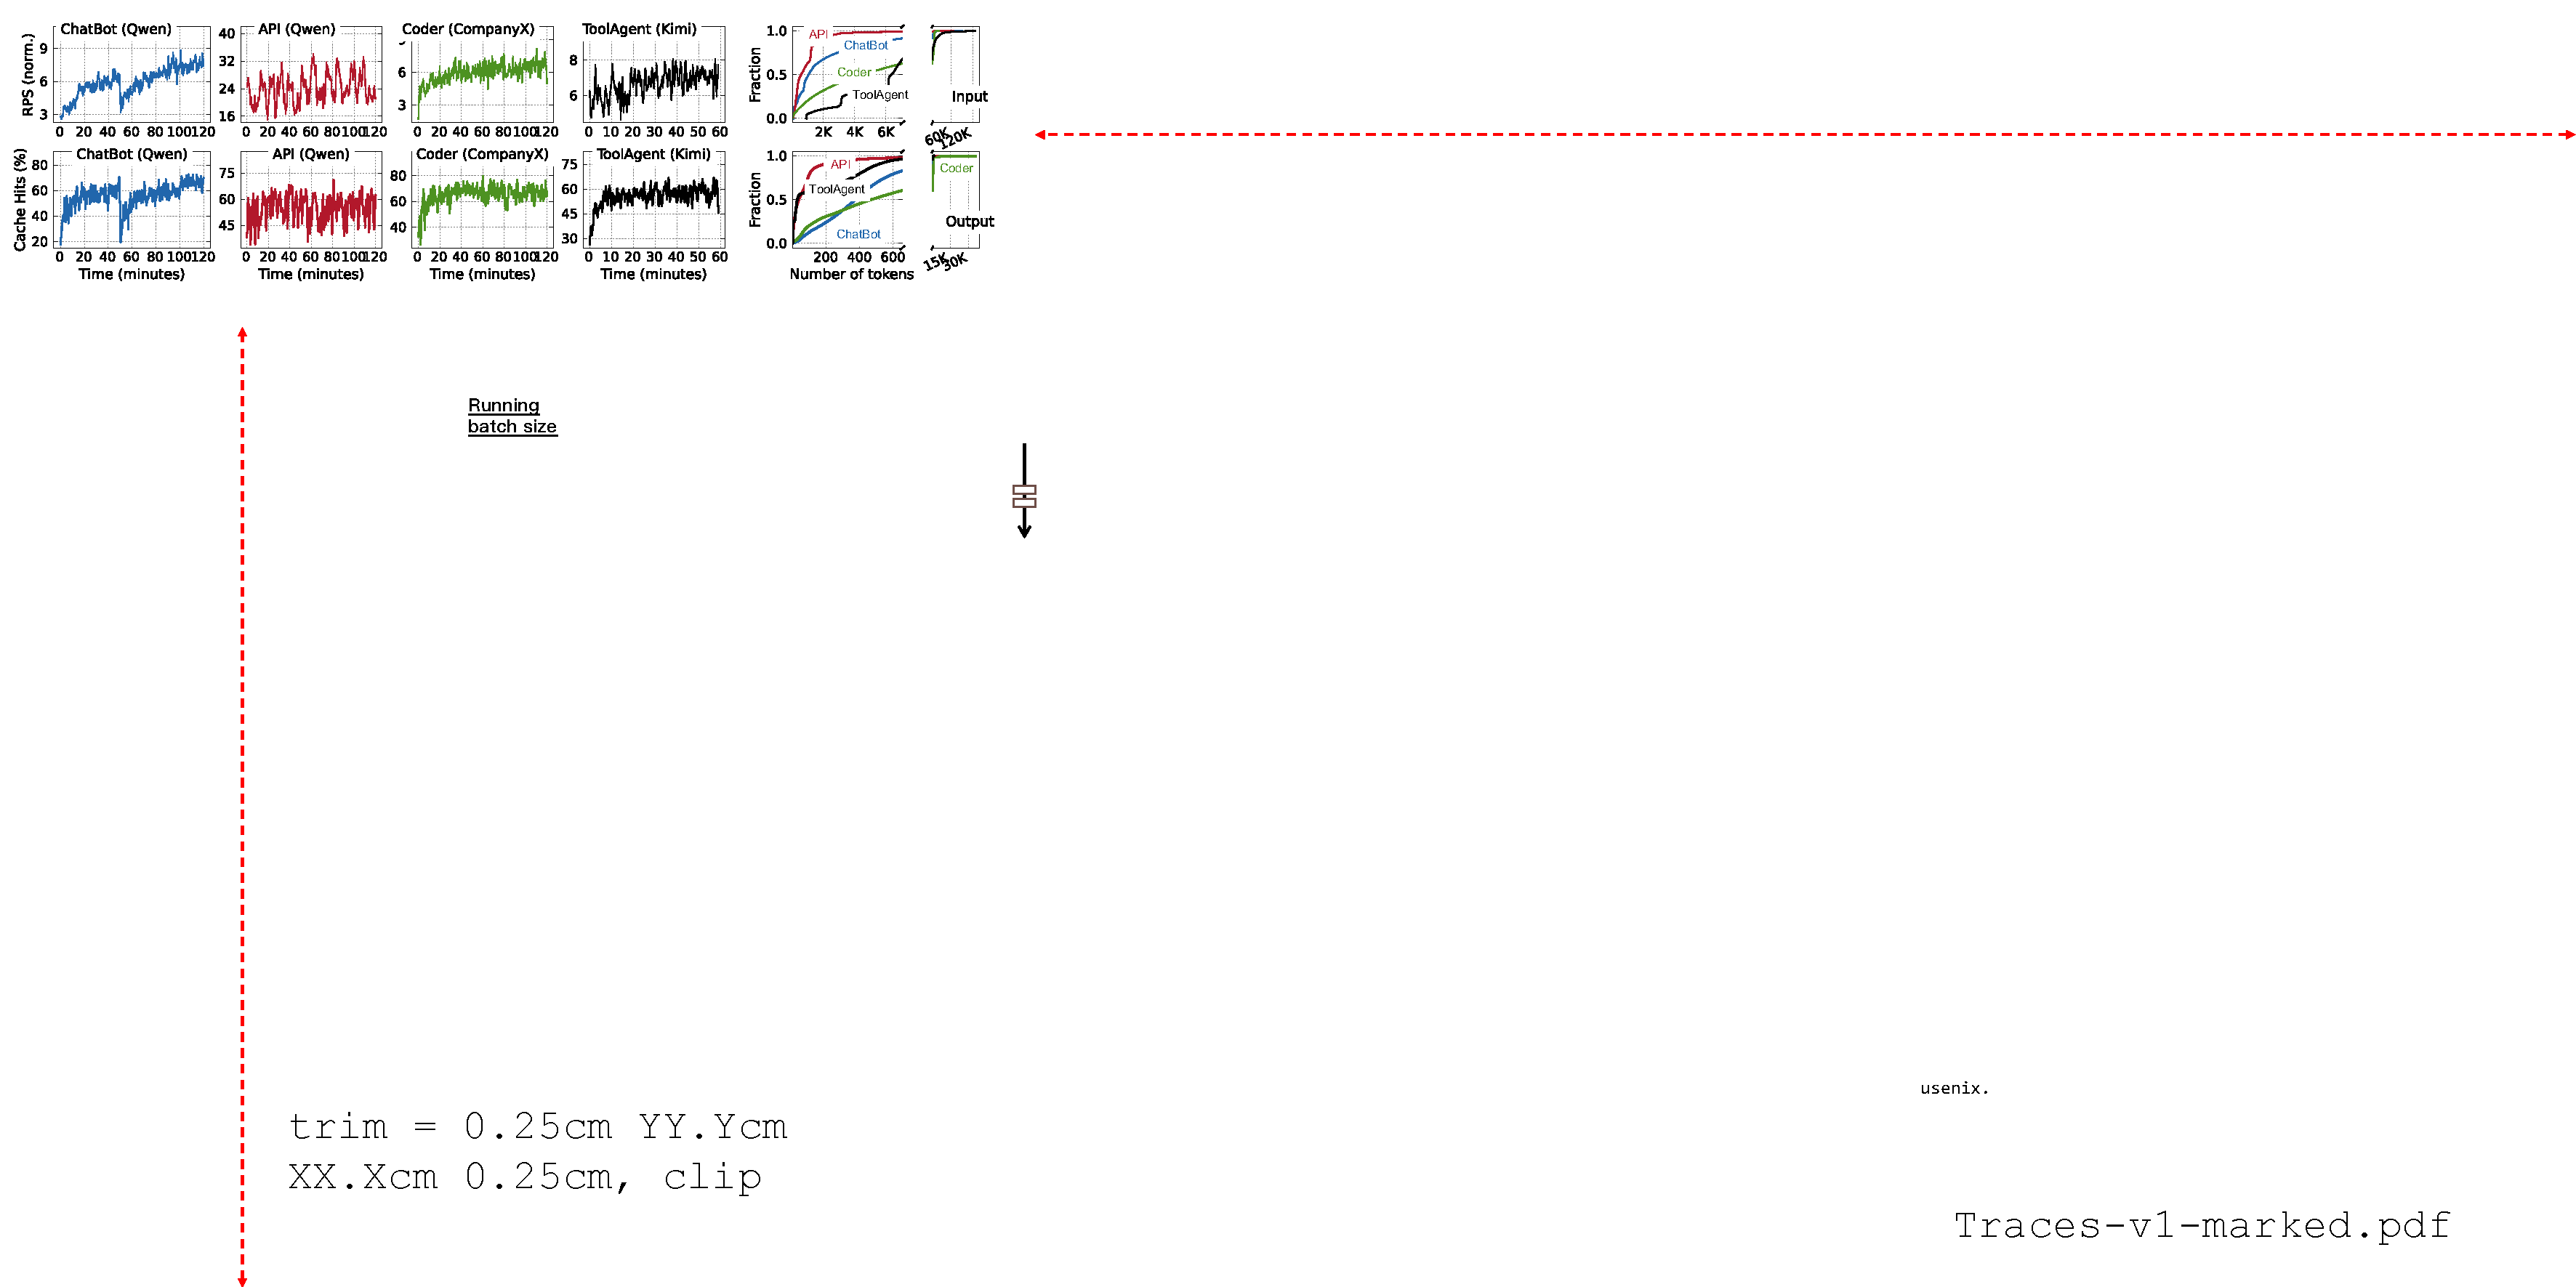
\includegraphics[width=0.99\linewidth, trim=0.25cm 22.45cm 36cm 0.25cm, clip]{figs/motiv/traces-v1-marked.pdf} \\[-18pt]
    \begin{minipage}{1\linewidth}
    \caption{\small{
       Our studied traces that cover major scenarios in powering LLM services.
        }}
    \label{fig:traces}
    \end{minipage} \\[-14pt]
\end{figure*}

\subsection{Characterization Methodology}
\label{sec:eval-setup}

\nospacestitle{Testbed and instance used. \,}
Without explicit mention, we conduct all our experiments
on a testbed containing 16 NVIDIA H20 GPUs---hardware similar to that used for hosting LLM services at {\company}.
Each GPU has 96\,GB HBM, which is sufficient for hosting common models available on the market~\cite{DBLP:conf/sosp/Xiang0QYZYZL0025}.
The router is deployed on a high-end CPU server with 160 Intel Xeon cores
and 1\,TB of DRAM.
Our instance runs the latest vLLM-v1 (vLLM)~\cite{vllm-code}---the state-of-the-art LLM serving engine
with the latest optimizations, such as chunked prefill~\cite{298679} and fast GPU kernels~\cite{flashinfer}.

\stitle{Models. \,} 
We chose LLM models that are representative of different architectures and popular choices on the market,
including dense (Qwen2-7B) and mixture-of-experts (MoE) models (Qwen3-30B)~\cite{DBLP:conf/sosp/Xiang0QYZYZL0025}. 

\stitle{Workloads. \,}
We conduct analyses on real-world LLM serving traces, both open-source and collected from {\company},
and cover common LLM applications:
\textbf{ChatBot (Qwen)} and \textbf{Agent (Qwen)}~\cite{bailian}
are open-sourced traces from Alibaba Cloud that
collect requests sent from a chatbot service similar to ChatGPT and
an LLM API calling agent service~\cite{claudeapi,geminiapi,openaiapi}, respectively.
\textbf{Coder} collects requests issued by coding copilot services to a dedicated cluster
in {\company} on a single day in November 2025, 
and \textbf{ToolAgent (Kimi)}~\cite{mooncake-trace} is another open-sourced trace from Kimi
that also collects requests from an agent service.
For traces except ToolAgent (Kimi),
they are all collected from a single cluster routed by one global router. 
ToolAgent (Kimi) does not mention how the trace is collected. 

Our analyzed workloads are representative---not
only because of the breadth of application scenarios chosen,
but also because each selected trace preserves the essential characteristics for evaluating
LLM scheduling policies.
Specifically, all requests in our traces contain the (hashed) content and the timestamp of the request issuance,
which are critical for evaluating the impact of {\kvcache}-aware scheduling on global scheduling (see \textsection{\ref{sec:kvcache-aware}}).
Other popular datasets like AzureLLMTrace~\cite{AzurePublicDataset} or BurstGPT~\cite{wang2025burstgpt} do not provide
such content.
Note that with traces containing hashed content, 
we can still replay it 
with behavior that exactly matches the original one by
reconstructing inputs according to the hash value,
and each instance executes the same number of decodes as in the traces regardless of the EOS token~\cite{kvcache}.
%Moreover, each request in our traces contains the timestamp of the request issuance,
%which more faithfully reflects real-world workload behavior than simulating arrival patterns with probability distributions~\cite{traceupscaler}.

{\fig{fig:traces}} visualizes key features of our evaluated traces,
including their request arrival rates, input and output token numbers,
and the {\kvcache} hit rates assuming an infinite {\kvcache} cache space.
Note that the request arrival rate is normalized due to confidentiality considerations
required for the \textbf{Coder} trace. 
For all these traces, we observe that over a given serving interval (e.g., 1 hour),
the request arrival and {\kvcache} hit rates are relatively stable, with a few short-term fluctuations.
Besides, though the input and output token numbers vary across traces, 
they are typically not so large except for a few outliers. 


\stitle{Trace scaling. \,}
Since the traces are collected from clusters with different scales than our testbed,
we scale the traces according to our testbed capability 
similar to prior work~\cite{DBLP:conf/asplos/MiaoSDXL0J24,DBLP:journals/pvldb/AliPYS22,DBLP:conf/osdi/GujaratiKAHKVM20,DBLP:conf/osdi/ZhangWLWS0025,traceupscaler}.
Without explicit mention, we scale the average request arrival rate to
half of the maximum rate of our testbed obtained via offline profiling.
This approximates the serving configurations in {\company} because
if the arrival rate approaches the serving capacity,
a common practice in {\company} is to reroute the requests to another
underloaded cluster,
 or simply reject them in non-critical cases (like ChatAPP)~\cite{305212}. 
Otherwise, the service-level objectives (SLOs) of many requests cannot be met due to queuing~\cite{queuing}.
Our end-to-end analysis in \textsection{\ref{sec:eval}} further measures
the impact of different request arrival rates on scheduling performance,
and shows consistent results.


\subsection{Load-balancing Alone is Insufficient for LLM}
\label{sec:kvcache-aware}

\begin{figure}[!t]
%    \hspace{1mm}
    \centering
%    \includegraphics[width=1\textwidth]{./figs/motiv/traces-v1.pdf}\\[-2pt]
     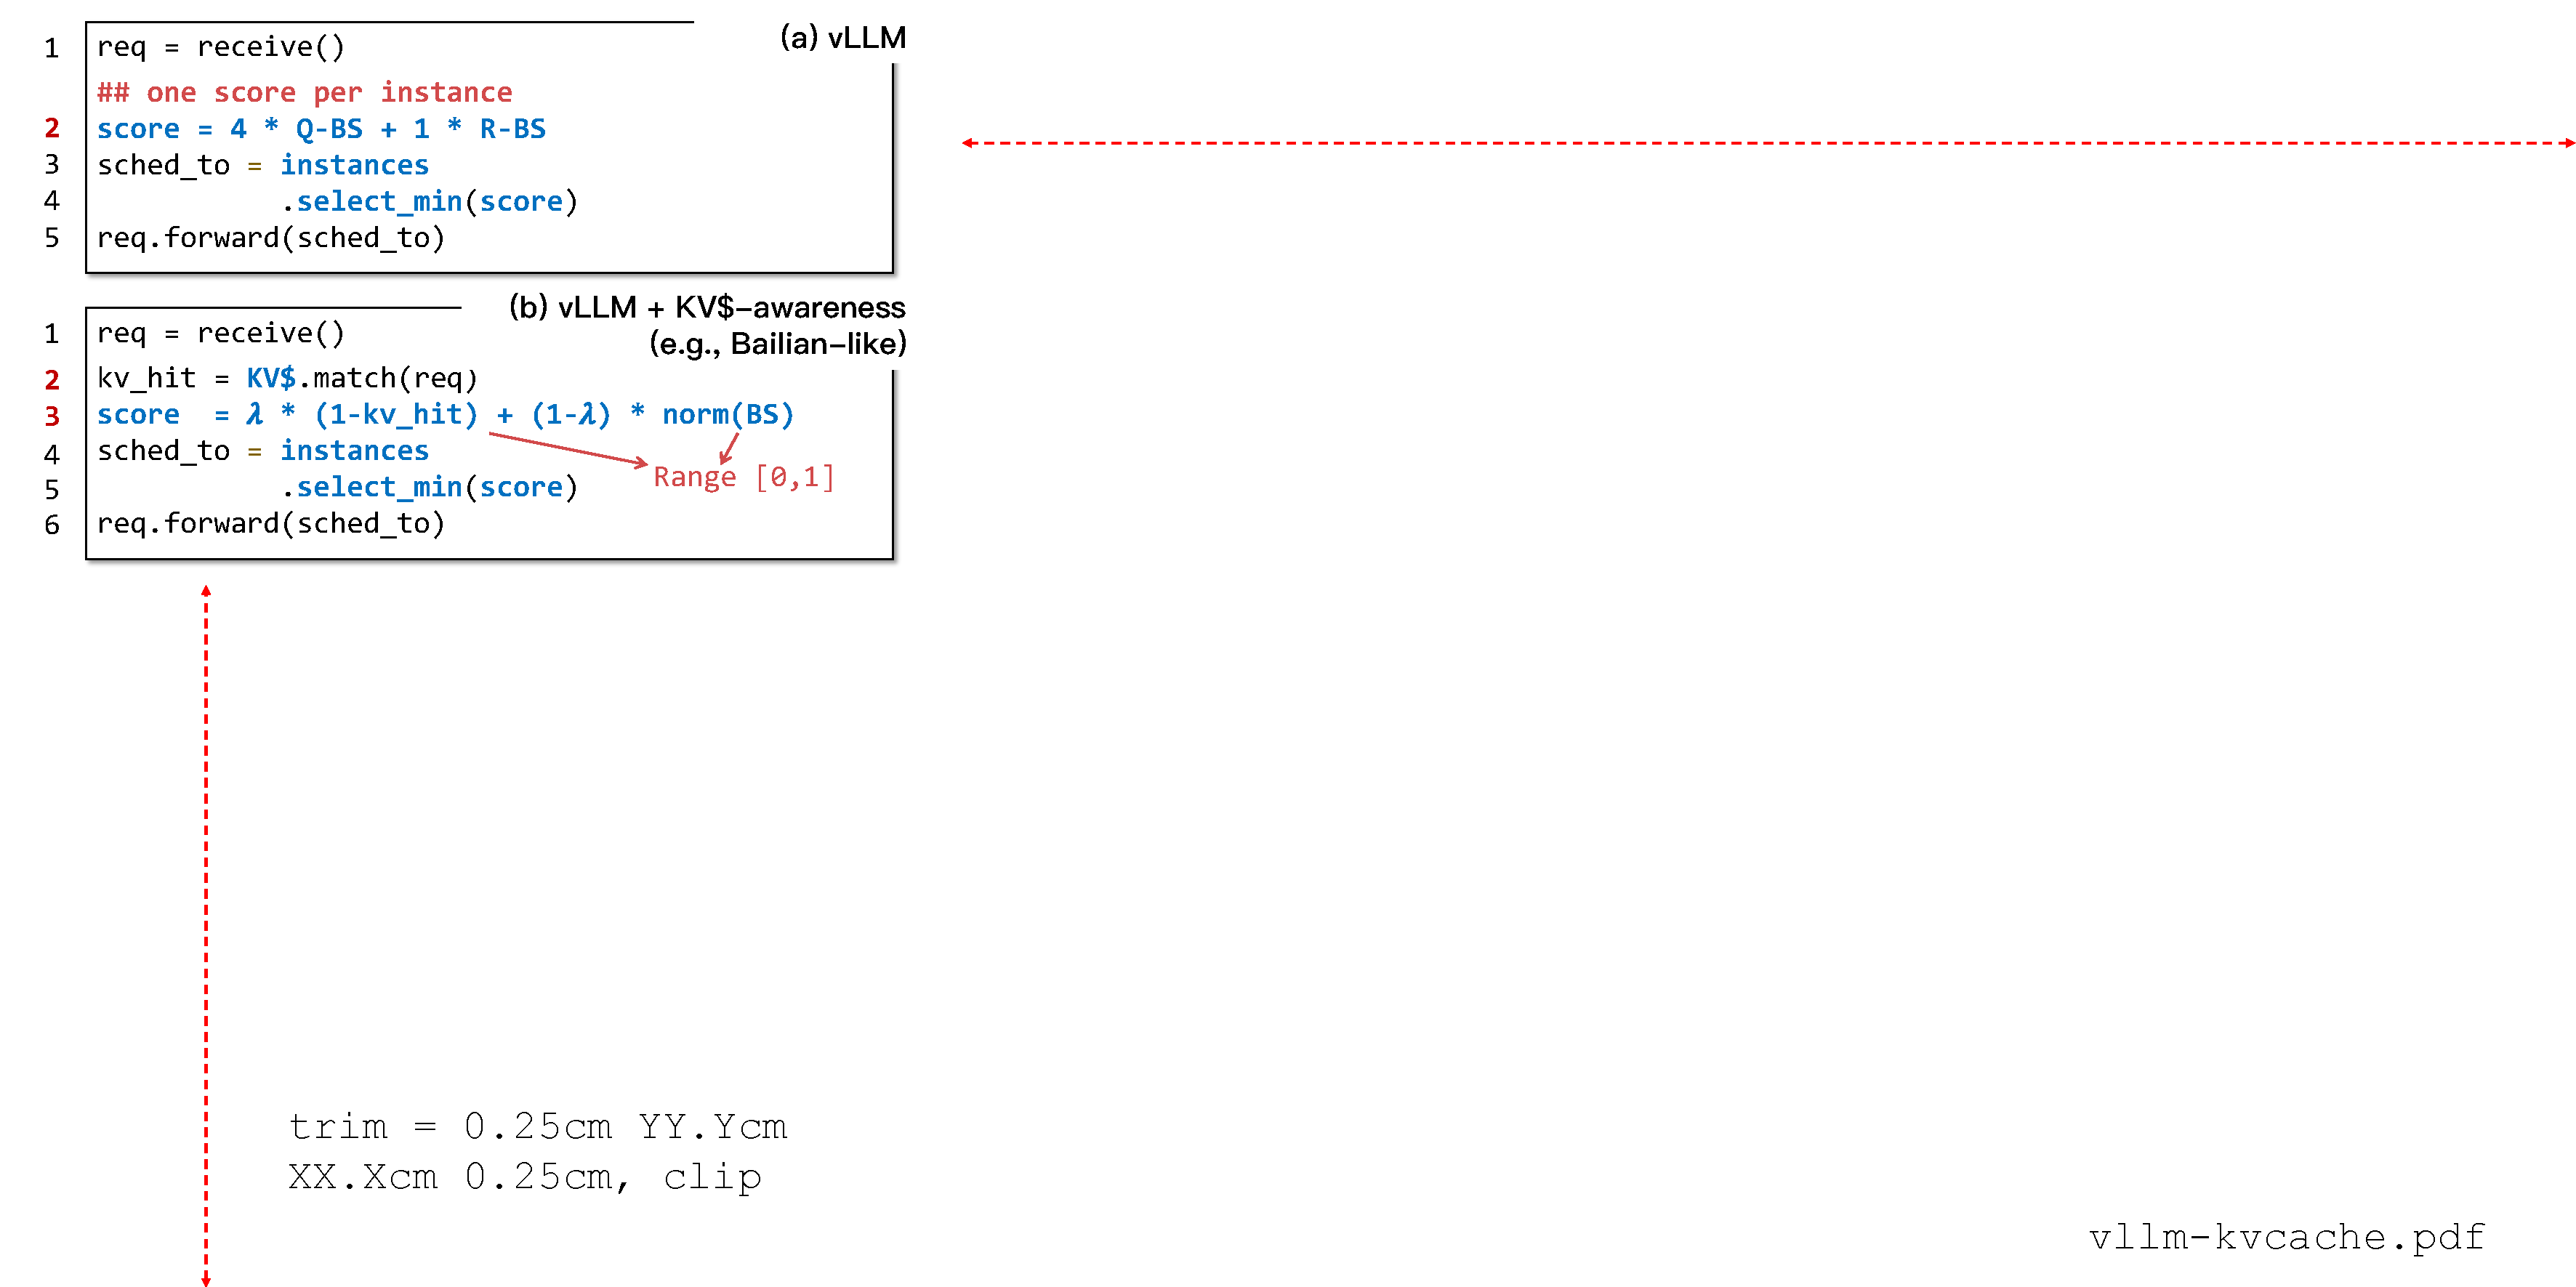
\includegraphics[width=0.9\linewidth, trim=0.25cm 16.4cm 37.65cm 0.25cm, clip]{figs/vllm-kvcache-v1.pdf} \\[5pt]
    \begin{minipage}{1\linewidth}
    \caption{\small{
        (a) The scheduling score of vLLM and 
        (b) adding {\kvcache}-awareness to its score for LLM scheduling. 
        Note that the linear combination of two indicators has only one degree of freedom (the weight $\lambda$).
        }}
    \label{fig:vllm-kvcache}
    \end{minipage} \\[-10pt]
\end{figure}

\begin{figure}[!t]
    \centering
    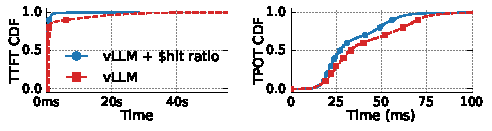
\includegraphics[width=1.0\linewidth]{figs/4-2-kvcache-aware/4-2-kvcache-aware-cdf-1-no-tail.pdf} \\[-0pt]
    \begin{minipage}{1\linewidth}
    \caption{\small{   
        A comparison of the performance of vLLM and KV cache-aware scheduling on ChatBot Trace with Qwen3-30B model.
        Other workloads and models are similar.
    }}
    \label{fig:kvcache-aware-cdf-1}
    \end{minipage} \\[-10pt]
\end{figure} 

\begin{figure}[t]
    \centering
    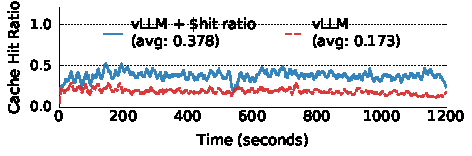
\includegraphics[width=0.97\linewidth]{./figs/4-2-kvcache-aware/kvcache-hit-timeline.pdf} \\[0pt]
    \begin{minipage}{1\linewidth}
    \caption{\small{A {\kvcache} hit ratio comparison of vLLM vs. {\kvcache}-aware scheduling on ChatBot Trace with Qwen3-30B model.
    Other workloads and models are similar.
    }}    
    \label{fig:kvcache-aware-hit-ratio1}
     \end{minipage} \\[-5pt]
\end{figure}


\begin{figure}[t]
    \centering
    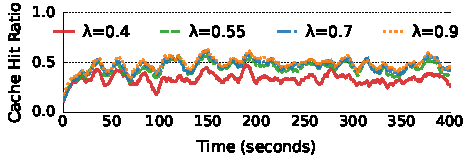
\includegraphics[width=0.97\linewidth]{figs/4-3-imbalance/4-2-cache-hit-t.pdf} \\[1pt]
     \begin{minipage}{1\linewidth}
    \caption{\small{
A comparison of the {\kvcache} hit ratio by changing the weight of {\kvcache}-awareness
in the policy described in {\fig{fig:vllm-kvcache}} (b) on ChatBot Trace with Qwen3-30B model.     
    }}
    \label{fig:chln-cache-hit}
    \end{minipage}
\end{figure}

\begin{figure}[!ht]
    \centering
    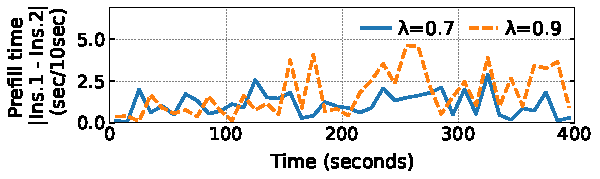
\includegraphics[width=0.98\linewidth]{figs/4-3-imbalance/4-3-pt-imbalance-absdiff.pdf} \\[-2pt]
    \caption{\small{
    A profile of the workload imbalance between two instances when running
    with two different weights in a linear combination on the ChatBot Trace using the Qwen3-30B model.
    The reported metric is the absolute served prefill time in each 10-second window
    between the two instances (Inst.).
    }}
    \label{fig:chln-pt-imbalance}
\end{figure}

\nospacestitle{A starting case: the vLLM policy~\cite{vllm-code}. \,}
Our study starts with the default global scheduling policy adopted by
vLLM~\cite{vllm-code}---a popular open-source LLM serving engine
widely used in both industry and academia.
{\fig{fig:vllm-kvcache}} (a) shows its scheduling method,
which uses the batch size of each instance as the indicator for the routing score.
It is essentially a variant of the classic load-balancing-centric join-the-shortest-queue (JSQ) policy
with an extension for LLM: at each instance,
the batch size includes both the requests running on the instance (R-BS)
and those queued in the instance's queue (Q-BS).

\begin{figure*}[!t]
%    \hspace{1mm}
    \centering
%    \includegraphics[width=1\textwidth]{./figs/motiv/traces-v1.pdf}\\[-2pt]
     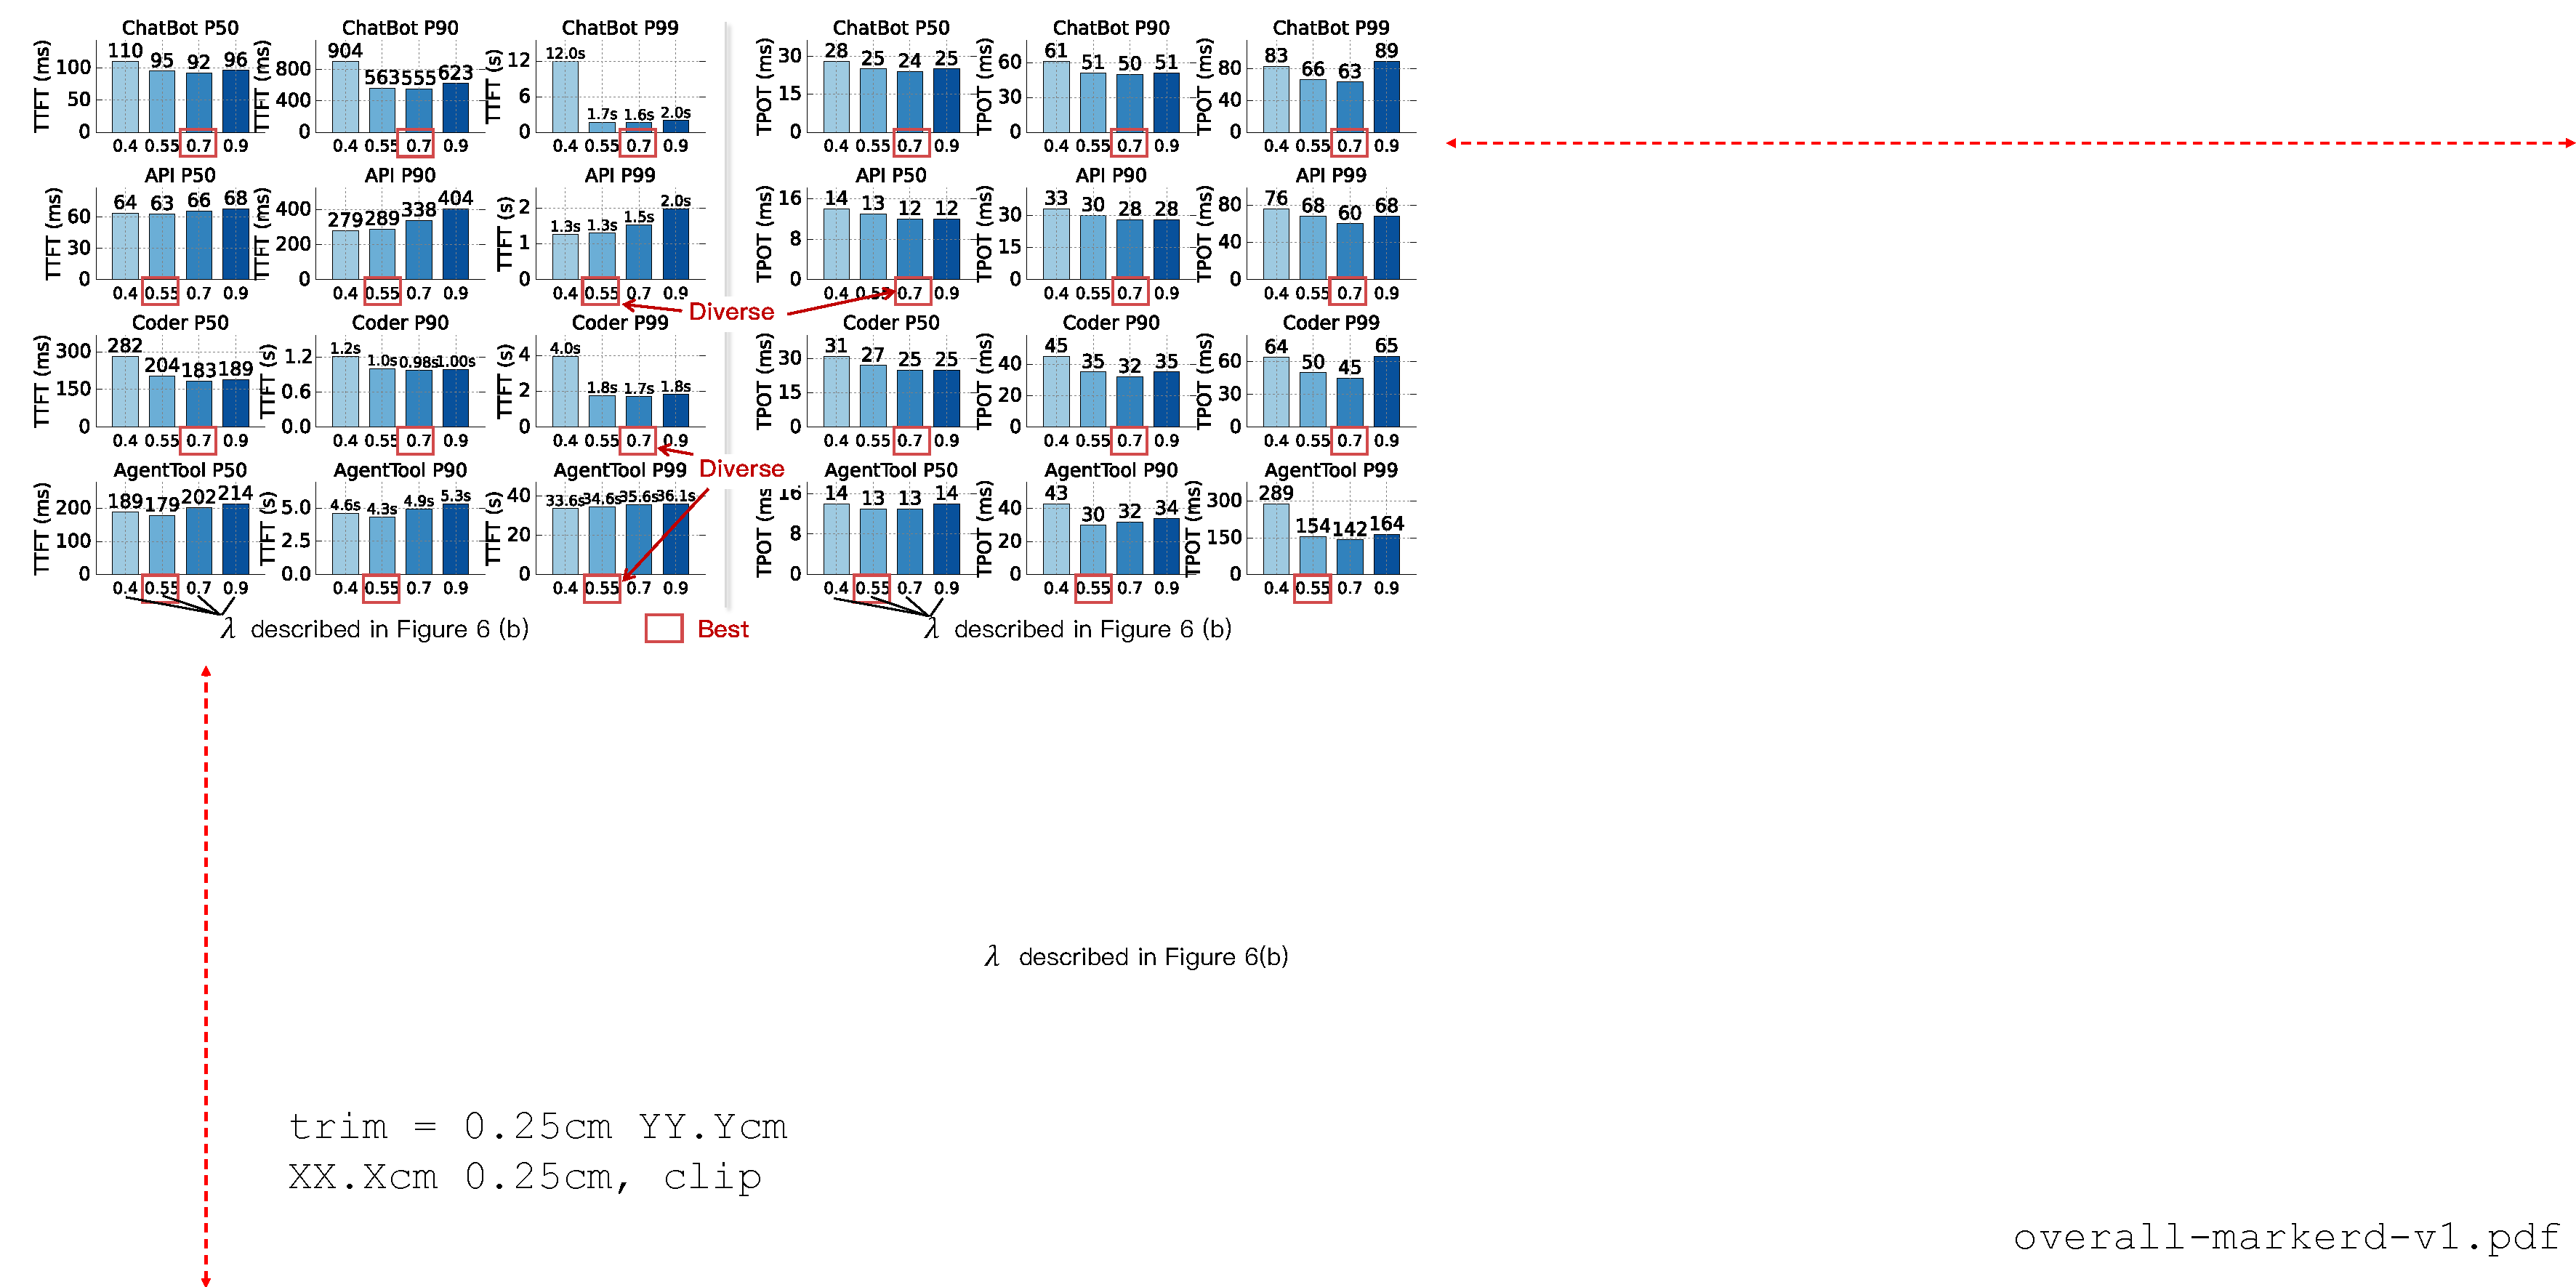
\includegraphics[width=0.95\linewidth, trim=0.25cm 14.52cm 26.5cm 0.25cm, clip]{figs/lambda-bar-chart/overall-marked-v1.pdf} \\[0pt]
    \begin{minipage}{1\linewidth}
    \caption{\small{
        An analysis of how the performance 
        varies with different hyperparameters on 
        four traces with linear-combination-based method. 
        The model used is Qwen3-30B. 
        }}
    \label{fig:data-linear-tune}
    \end{minipage} \\[-10pt]
\end{figure*}

\stitle{Retrofitting vLLM with {\kvcache}-awareness (\company). \,} 
While JSQ tries to balance the workload across instances,
it is unaware of the {\kvcache} state of the incoming requests.
That is, routing requests to instances with a higher {\kvcache} hit rate
substantially reduces request latency.
{\fig{fig:vllm-kvcache}} (b) shows a simple extension of vLLM
adopted by {\company} and others~\cite{ai-Dynamo,aigw} to make request scheduling {\kvcache}-aware:
it adds a {\kvcache} indicator to the score function---a ratio
that estimates the {\kvcache} hit ratio if the request is routed to that instance.
Note that $KV$ is the symbolic value representing the per-instance {\kvcache} hash map.
There are two points to note here:
(1) the load balance indicator (batch size) needs to be normalized to $[0,1]$
to match the scale of the hit ratio because otherwise
they cannot simply be added together;
(2) the analysis in this section assumes the linear combination coefficients ($\lambda$) are fixed,
and the next section discusses the rationale for setting them.


As shown in {\fig{fig:kvcache-aware-cdf-1}}, 
adding {\kvcache}-awareness to a load-balancing-only policy 
improves the average TTFT by 84\% and the average TPOT by 17\%, 
which is as expected because 
it increases the {\kvcache} hit ratio as profiled in {\fig{fig:kvcache-aware-hit-ratio1}}. 
Interestingly, although the improved {\kvcache} hit ratio---at a first glance---is only 
beneficial to the prefill, 
we found it is also helpful to the decode time 
because it reduces the computation required for each instance, 
allowing the instance to dedicate more GPU time to the decode phase.


\subsection{{\kvcache}-awareness vs. Load balancing: The Trade-off}
\label{sec:challenge-balancing}

\iffalse
\begin{figure}[t]
    \centering
    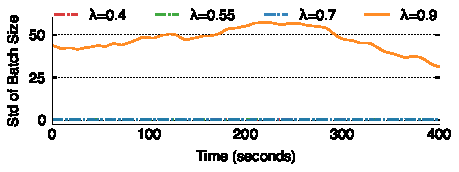
\includegraphics[width=1.0\linewidth]{figs/4-3-imbalance/batch_size_std_all_strategies.pdf}
    \caption{\small{Std of batchsize of different routing policies during contiguous burst periods}}
    \label{fig:chln-bs-imbalance}
\end{figure}
\fi

\iffalse
\begin{figure}[t]
    \centering
    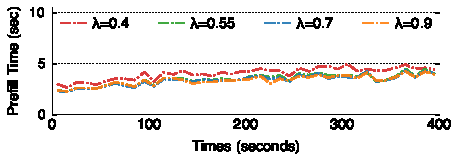
\includegraphics[width=1.0\linewidth]{figs/4-3-imbalance/prefill_time_per_10_secs_avg.pdf}
    \caption{\small{Average perfill time among instances every 10-seconds during contiguous burst periods}}
    \label{fig:chln-avg-pt}
\end{figure}
\fi


\noindent
While intuitive, integrating {\kvcache}-awareness into the system is non-trivial.
The root cause is that considering {\kvcache}-awareness may interfere with load balancing.
Specifically,
when defining scores with a linear combination as described previously,
the priority of the considered objective is controlled
by the weight assigned to each indicator in the scoring function ($\lambda=0.4$) in {\fig{fig:vllm-kvcache}} (b):
if we assign a larger weight to the {\kvcache} component,
the router will prioritize routing requests to instances with higher {\kvcache} hit ratios,
even though other instances may have a much lower load.
This, on the other hand, may lead to load imbalance across instances.

{\fig{fig:data-linear-tune}} illustrates this trade-off by presenting the overall TTFT and TPOT 
of using a linear combination of described in the previous section ({\fig{fig:vllm-kvcache}} (b)) 
with various weights on the {\kvcache}-awareness component. 
We can see that when increasing the weight from 0.4 to 0.9, the
TTFT first gradually decreases and then increases except for the
API trace, which has less impact due to its short input length. 

To demystify the trend observed with the trade-off,
{\fig{fig:chln-cache-hit}} further shows the {\kvcache} hit ratio
when changing the weight of {\kvcache}-awareness on the ChatBot trace.
Other traces show similar trends.
We can clearly see that when increasing the {\kvcache} weight, the overall {\kvcache} hit ratio increases accordingly.
This explains the reduced TTFT when increasing the weight from 0.4 to 0.7. 

% On the other hand, when increasing the weight to a threshold (e.g., 0.7 for the ChatBot),
Despite the increased {\kvcache} hit ratio, there is a knee point in the weight (e.g., 0.7 for the ChatBot),
beyond which the overall latency starts to increase. 
This is due to load imbalance across instances and we have profiled this phenomenon in 
{\fig{fig:chln-pt-imbalance}}, which plots the prefill
work assigned to two instances
using different linear combined weights (0.7 vs. 0.9) for serving the same 400-second burst period using the ChatBot trace.
The prefill time refers to the number of seconds the instance spends on prefill within each 10-second window.
This is a good measure of workload assigned to each instance because intuitively,
most tokens are generated during the decode phase. Therefore, if the prefill time dominates the processing time
on an instance, that instance generates fewer tokens than others.
For each profiled setup, we select two instances (from a total of 16 instances)
with the highest standard deviation of prefill time for ease of presentation.
We observe that for setups with a higher {\kvcache} priority ($\lambda=0.9$),
the total prefill time differs significantly between the two instances.
In comparison, a balanced setup ($\lambda=0.7$) exhibits similar prefill times,
and during this period, the average prefill time is also similar.
Specifically, with $\lambda=0.7$, the average prefill time is 3.43s vs. 3.40s
for the two instances, whereas with $\lambda=0.9$, it is 3.57s vs. 2.17s.




\subsection{The Case of Linear Combination}
\label{sec:linear-combination}

\noindent
%While the linear combination method described in \textsection{\ref{sec:kvcache-aware}}
%can improve performance thanks to being {\kvcache}-aware,
%{\kvcache}-awareness requires non-trivial hyperparameter tuning to balance its interference
%with load balancing as we have described in the previous section, hence leading to two issues:
Based on the trade-offs explored previously, 
using a linear combination to achieve both {\kvcache}-awareness and load balancing leads to two issues:

\stitle{Cons \#1. Requires workload-specific hyperparameter tuning. \,}
The importance of {\kvcache} and its impact on load imbalance is workload-dependent.
For example, {\fig{fig:data-linear-tune}} presents the tuning results for different traces when running a Qwen3-30B model.
We can see that the evaluated optimal weight for each workload varies:
in ChatBot the optimal weight is 0.7, while in API it is 0.55,
even though both workloads have a similar {\kvcache} access pattern.
Note that we cannot afford to sweep all possible configurations,
as replaying each trace on the testbed consumes a substantial amount of GPU time.
As a result, the performance of the linear combination requires workload-specific hyperparameter tuning that 
is non-trivial in practice due to the diversity of workloads~\cite{10.5555/3768039.3768067}.


\stitle{Con \#2. Sub-optimal performance. \,}
During the evaluation in \textsection{\ref{sec:eval}}, 
we found that a statically tuned weight cannot always achieve competitive performance compared to other baselines. 
We hypothesize that this is because the optimal weight may vary over time; 
for example, the {\kvcache} hit pattern of different requests may change over time
 (see the second row of {\fig{fig:traces}}). 
 However, to the best of our knowledge, 
 all existing work uses a fixed tuned weight for the entire serving duration. 
 While it is possible to design strategies to adaptively tune the weight over time, 
 doing so would subsequently add system complexity.

 \iffalse
 \stitle{One side note: Regulation is important for the combinator. \,}
 \TODO{xx}
 \fi

\begin{figure*}[!t]
%    \hspace{1mm}
    \centering
%    \includegraphics[width=1\textwidth]{./figs/motiv/traces-v1.pdf}\\[-2pt]
     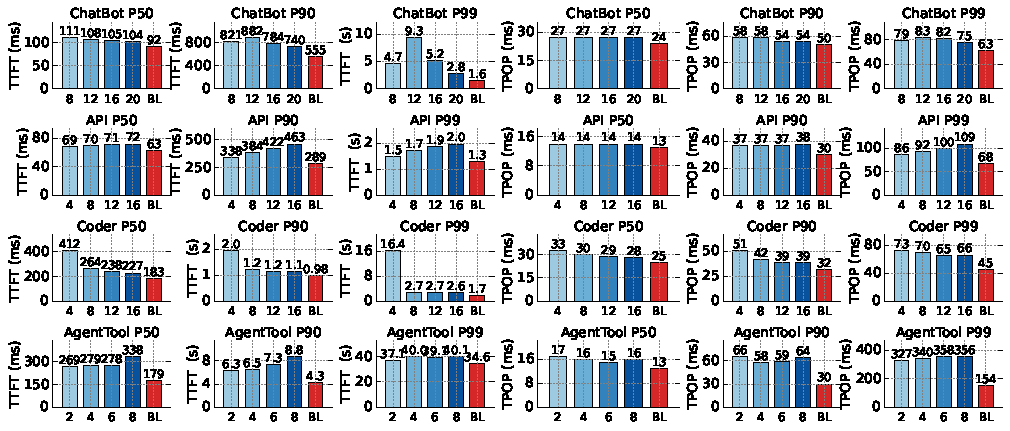
\includegraphics[width=0.99\linewidth]{figs/filter-based/overall-v1.pdf} \\[2pt]
    \begin{minipage}{1\linewidth}
    \caption{\small{
        An analysis of how performance
        varies with different hyperparameters on
        four traces using a filter-based combination method.
        \textbf{BL} denotes the \uline{l}inear-combination-based method for comparison, tuned with the \uline{b}est
        hyperparameter.
        The numbers (2,4,6,8) are the range described in {\fig{fig:aibrix}}.
        The model used is Qwen3-30B. 
        }}
    \label{fig:data-filter-tune}
    \end{minipage} \\[-10pt]
\end{figure*}

\subsection{The Case of Filter-based Combination}
\label{sec:filter-combination}

\begin{figure}[!t]
%    \hspace{1mm}
    \centering
%    \includegraphics[width=1\textwidth]{./figs/motiv/traces-v1.pdf}\\[-2pt]
     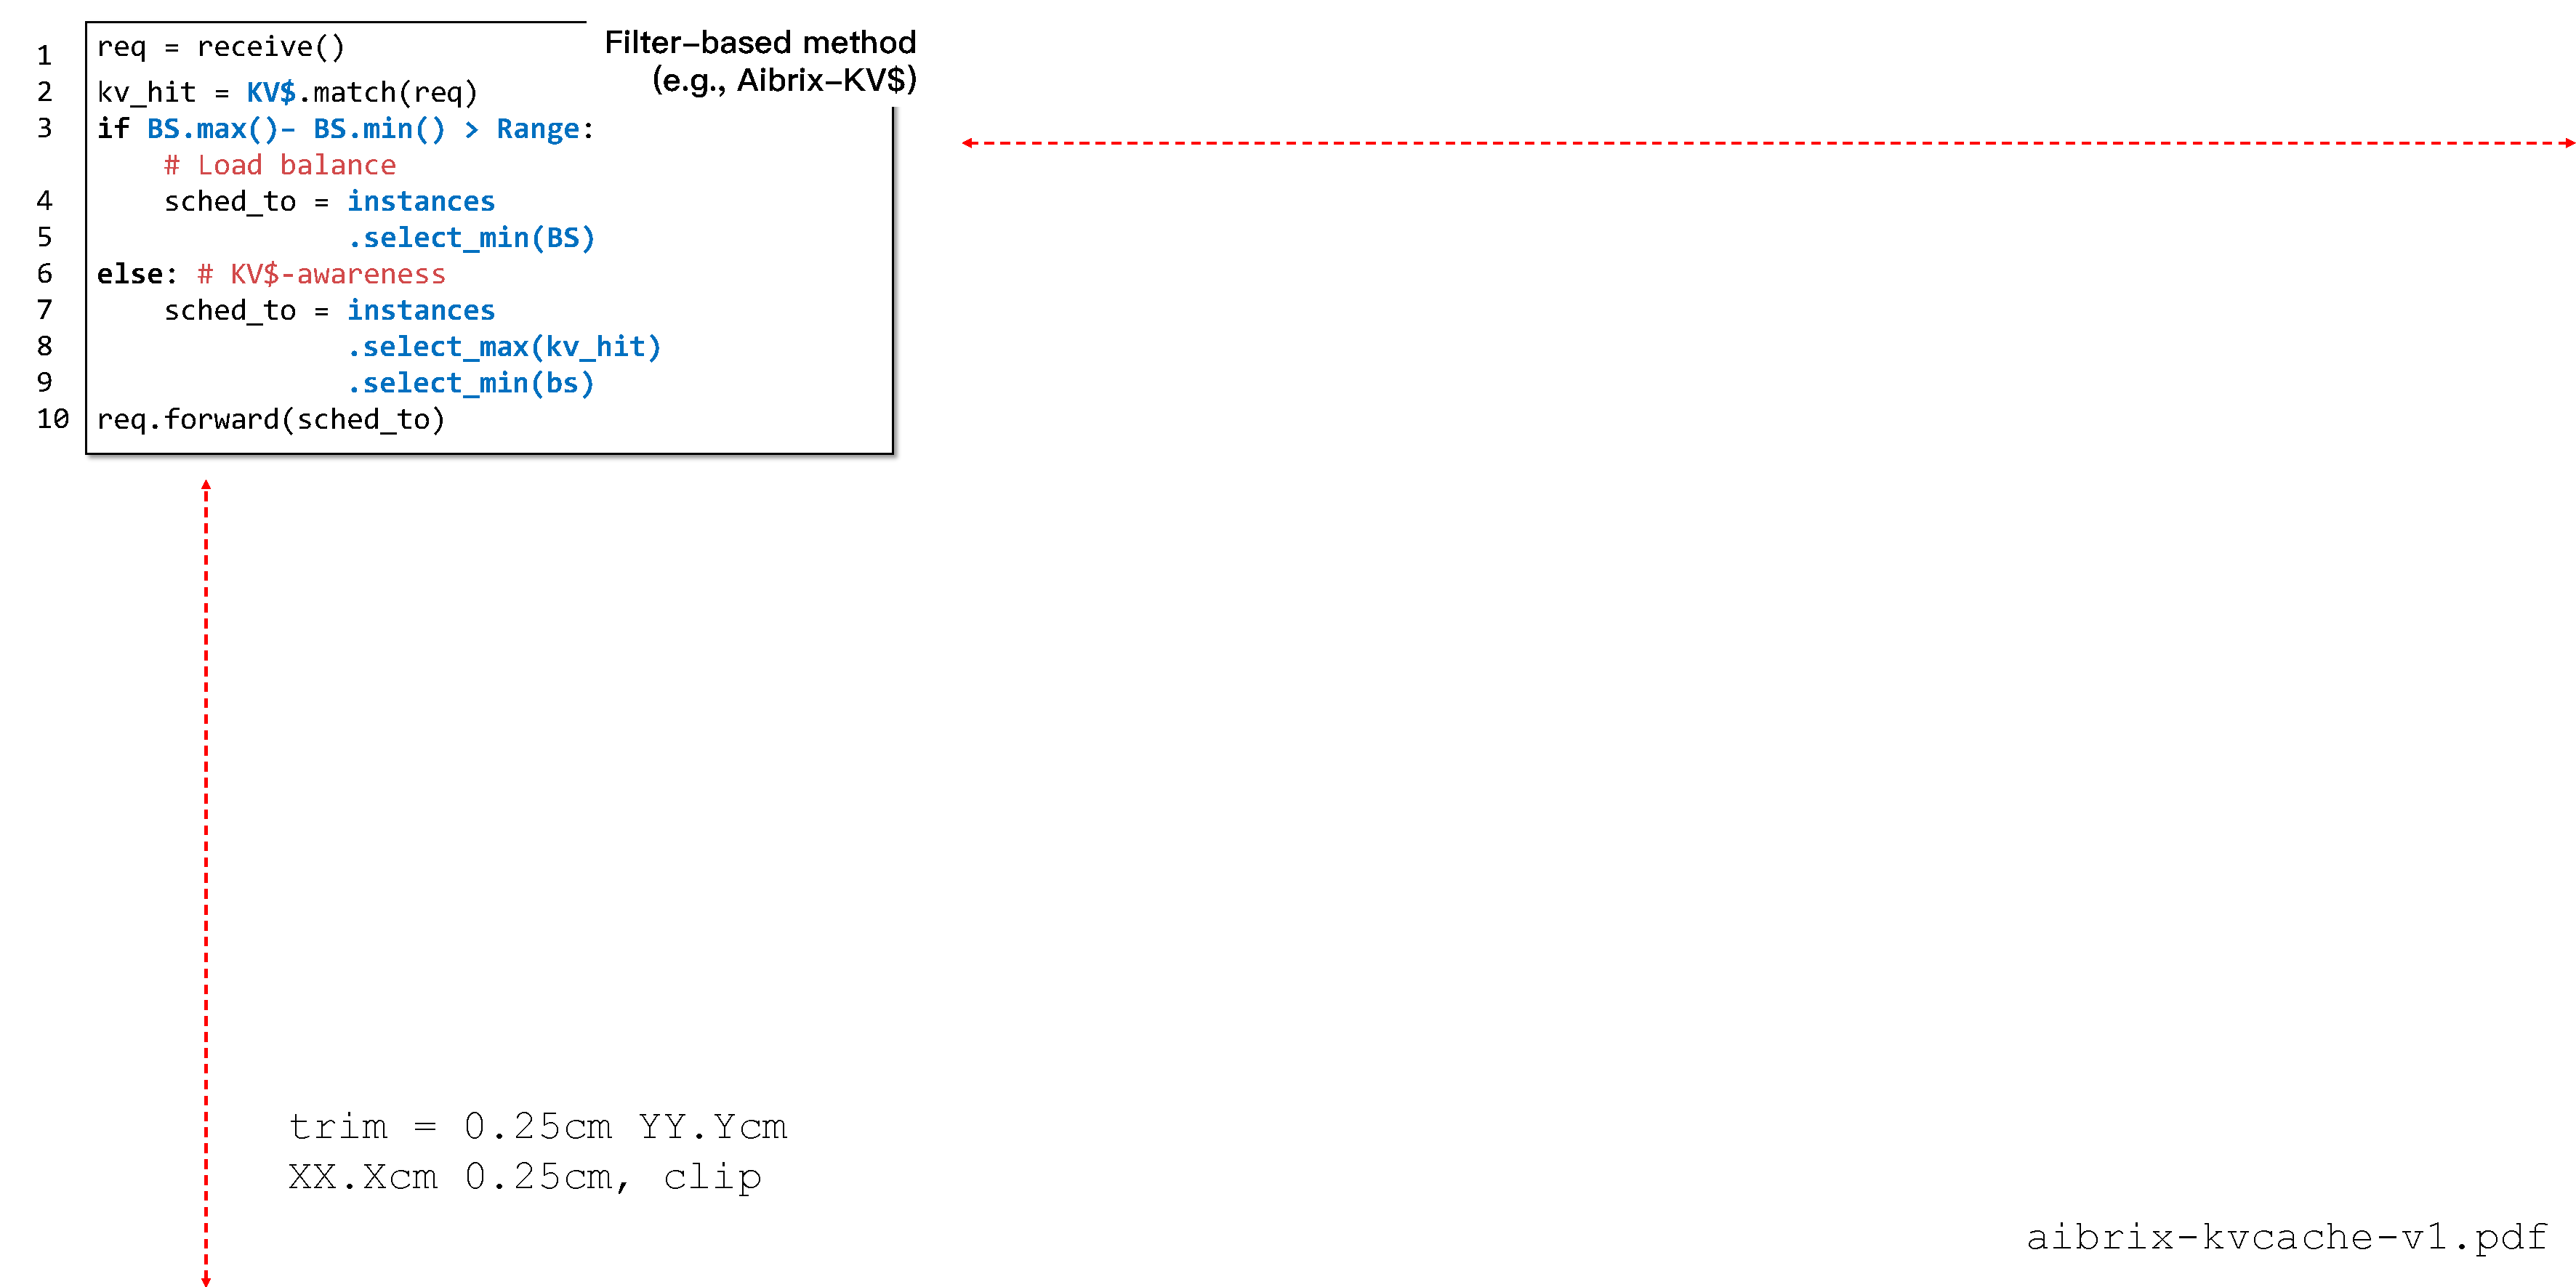
\includegraphics[width=0.9\linewidth, trim=0.25cm 18.9cm 37.65cm 0.25cm, clip]{figs/aibrix-kvcache-v1.pdf} \\[5pt]
    \begin{minipage}{1\linewidth}
    \caption{\small{
        The pseudocode of filter-based combination of {\kvcache}-awareness and load balancing in LLM scheduling,
        simplified from \texttt{prefix-cache} policy of AIBrix ~\cite{aibrix}. 
        }}
    \label{fig:aibrix}
    \end{minipage} \\[-10pt]
\end{figure}

\nospacestitle{Methodology. \,}
{\fig{fig:aibrix}} shows how a typical filter-based combination works for
integrating {\kvcache}-awareness and load balancing
in typical LLM scheduling systems like AIBrix~\cite{aibrix}.
First, the router checks whether the current cluster has an imbalanced load---i.e.,
the range between the maximum and minimum batch sizes across instances (\(\texttt{BS.max() - BS.min()}\)) exceeds a threshold (line 3).
If so, the router abandons {\kvcache}-awareness and simply routes the request to the instance
with the smallest batch size for load balancing (lines 4--5).
Otherwise, the router uses the {\kvcache} hit ratio as an indicator to route requests to instances (lines 6--9) for {\kvcache}-awareness.

\stitle{Cons \#1. Still require workload-specific hyperparameter tuning. \,}
Similar to linear combination, filter-based methods also require
hyperparameter tuning because the threshold for determining load imbalance (\texttt{Range})
is workload-dependent.
As shown in {\fig{fig:data-filter-tune}},
the optimal threshold of a typical filter-based method~\cite{aibrix} varies across workloads:
for example, in Coder, increasing the threshold from 4 to 16 improves
the P50 TTFT and TPOT by 44\% and 15\%, respectively. 
On the other hand, for the API trace 16 is a better choice than 4. 


\stitle{Cons \#2. Sub-optimal performance. \,}
Besides hyperparameter tuning, filter-based combination is slower
compared to linear combination with properly tuned weights,
as shown in {\fig{fig:data-filter-tune}}, 
because it biases towards load balancing and may forgo the benefits of {\kvcache}-awareness. 
Specifically, when a load imbalance is detected, it completely ignores {\kvcache}-awareness,
even though routing requests to instances with a higher {\kvcache} hit ratio could still be beneficial
if the amount of reduced computation is significant (as it helps reduce the load).
With linear combination, this is possible as long as the weight
assigned to the {\kvcache} hit ratio is not too small. 
This is not possible in filter-based methods. 

\subsection{The Case of Simulation-based Combination}
\label{sec:prediction-combination}
\begin{figure}[!t]
%    \hspace{1mm}
    \centering
%    \includegraphics[width=1\textwidth]{./figs/motiv/traces-v1.pdf}\\[-2pt]
    %  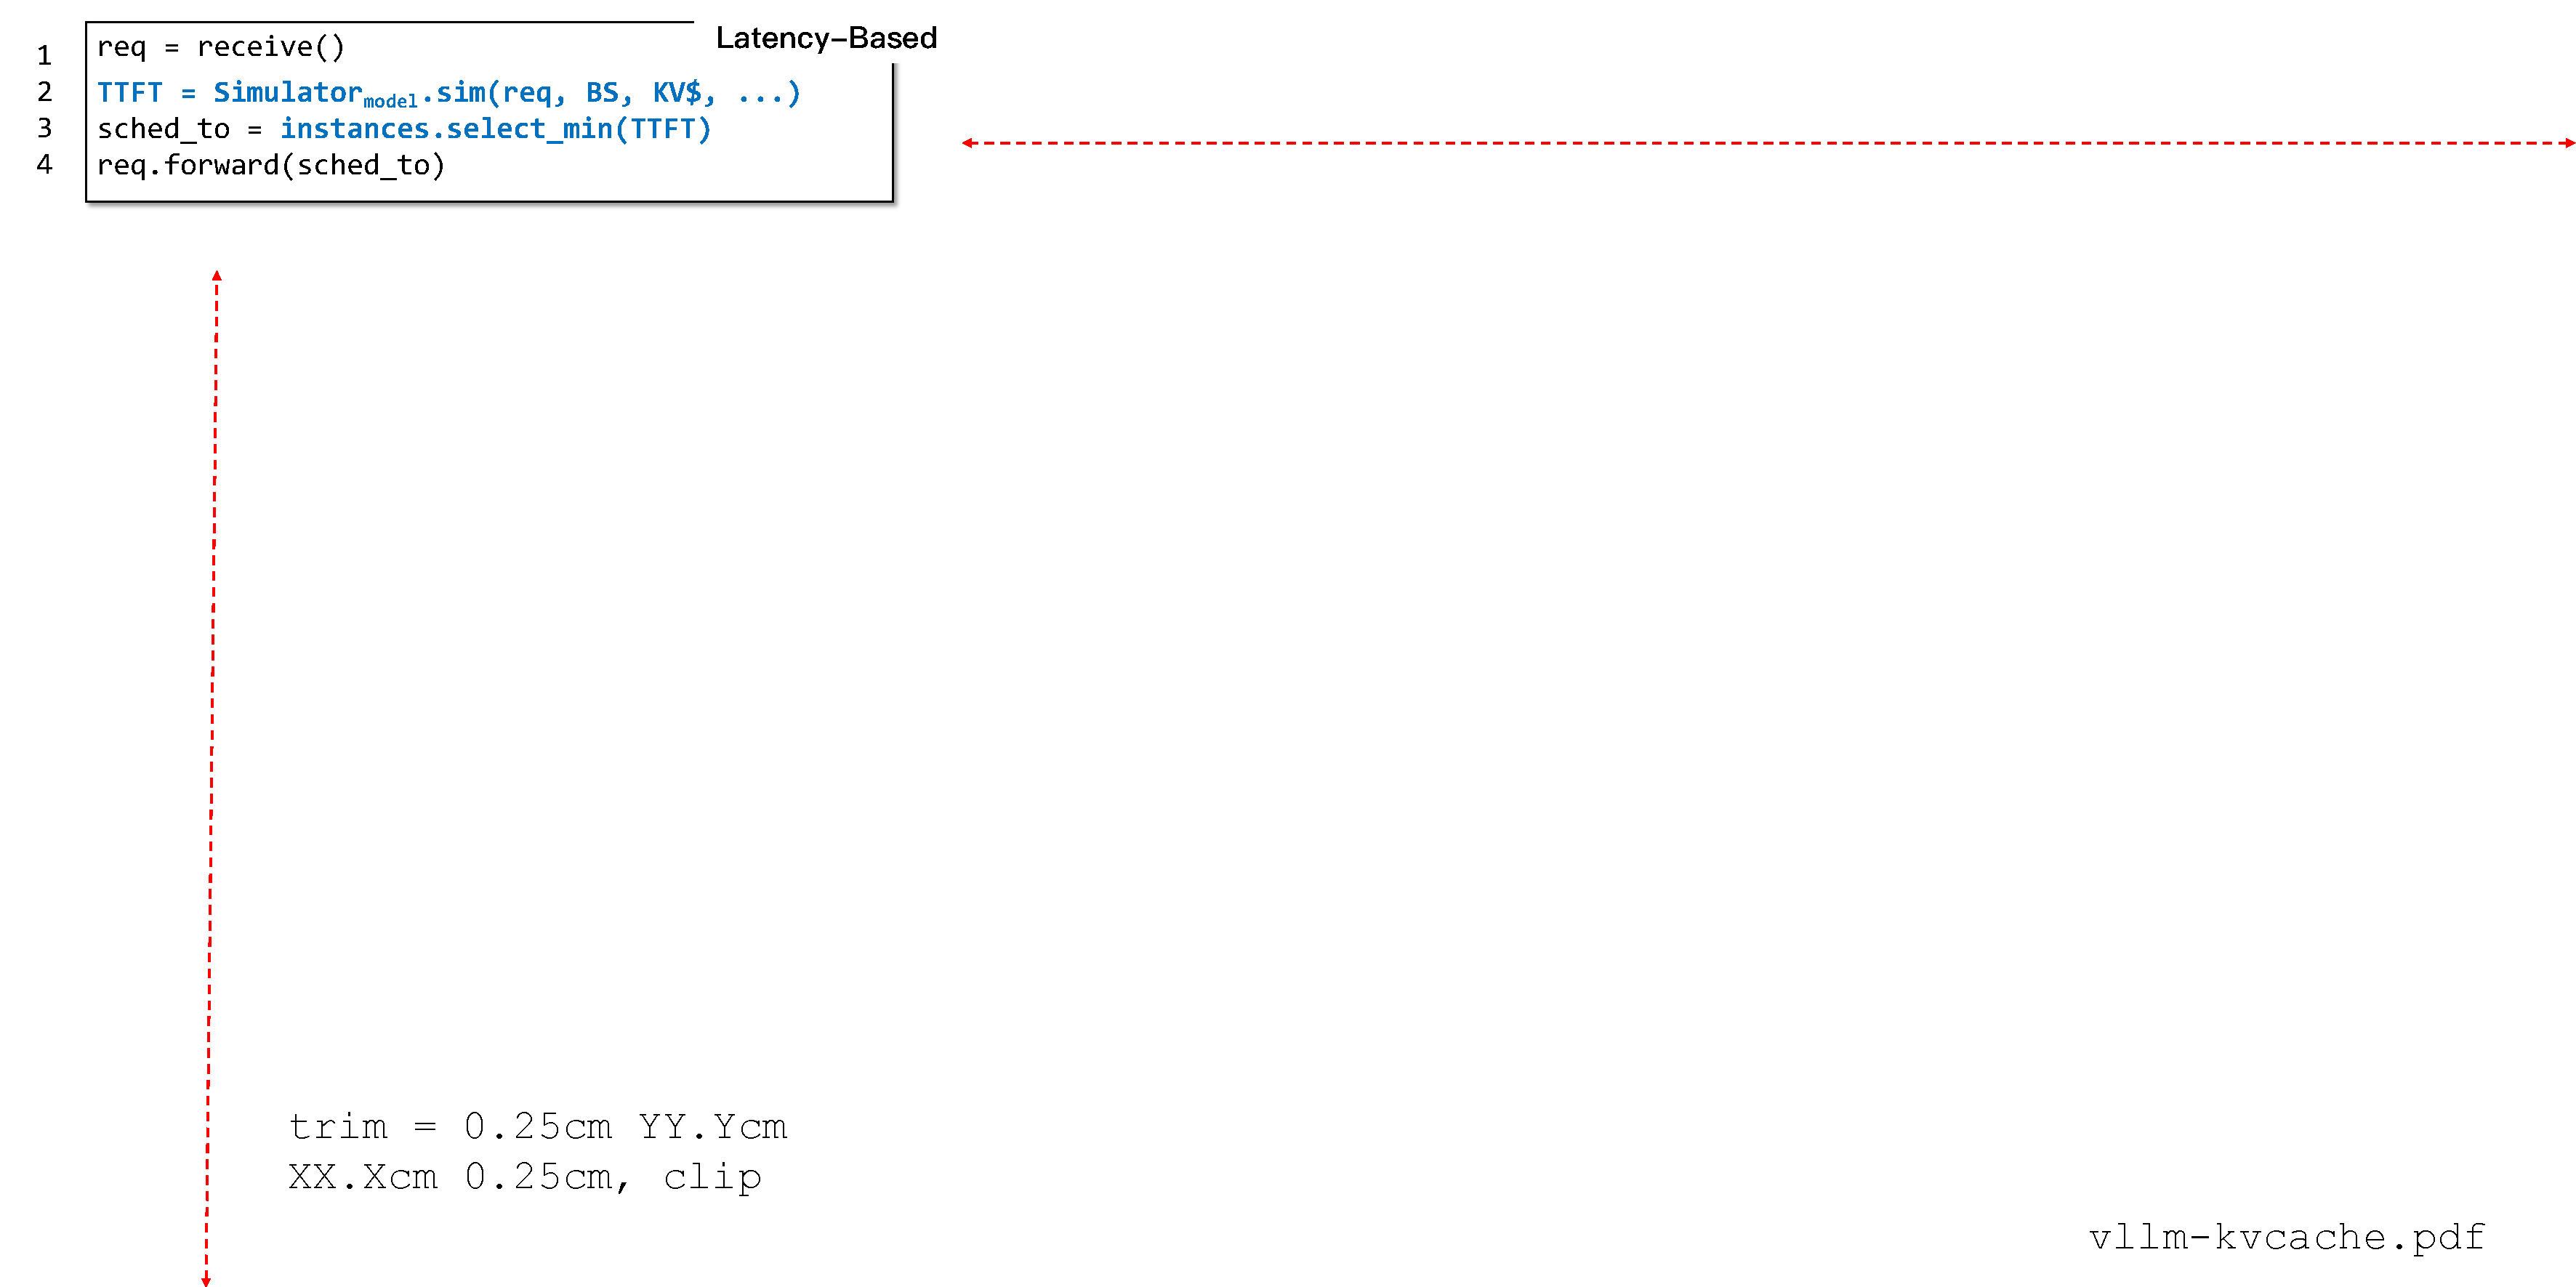
\includegraphics[width=0.96\linewidth, trim=0.25cm 14.5cm 41cm 0.25cm, clip]{figs/latency-based-v1.pdf} \\[-2pt]
     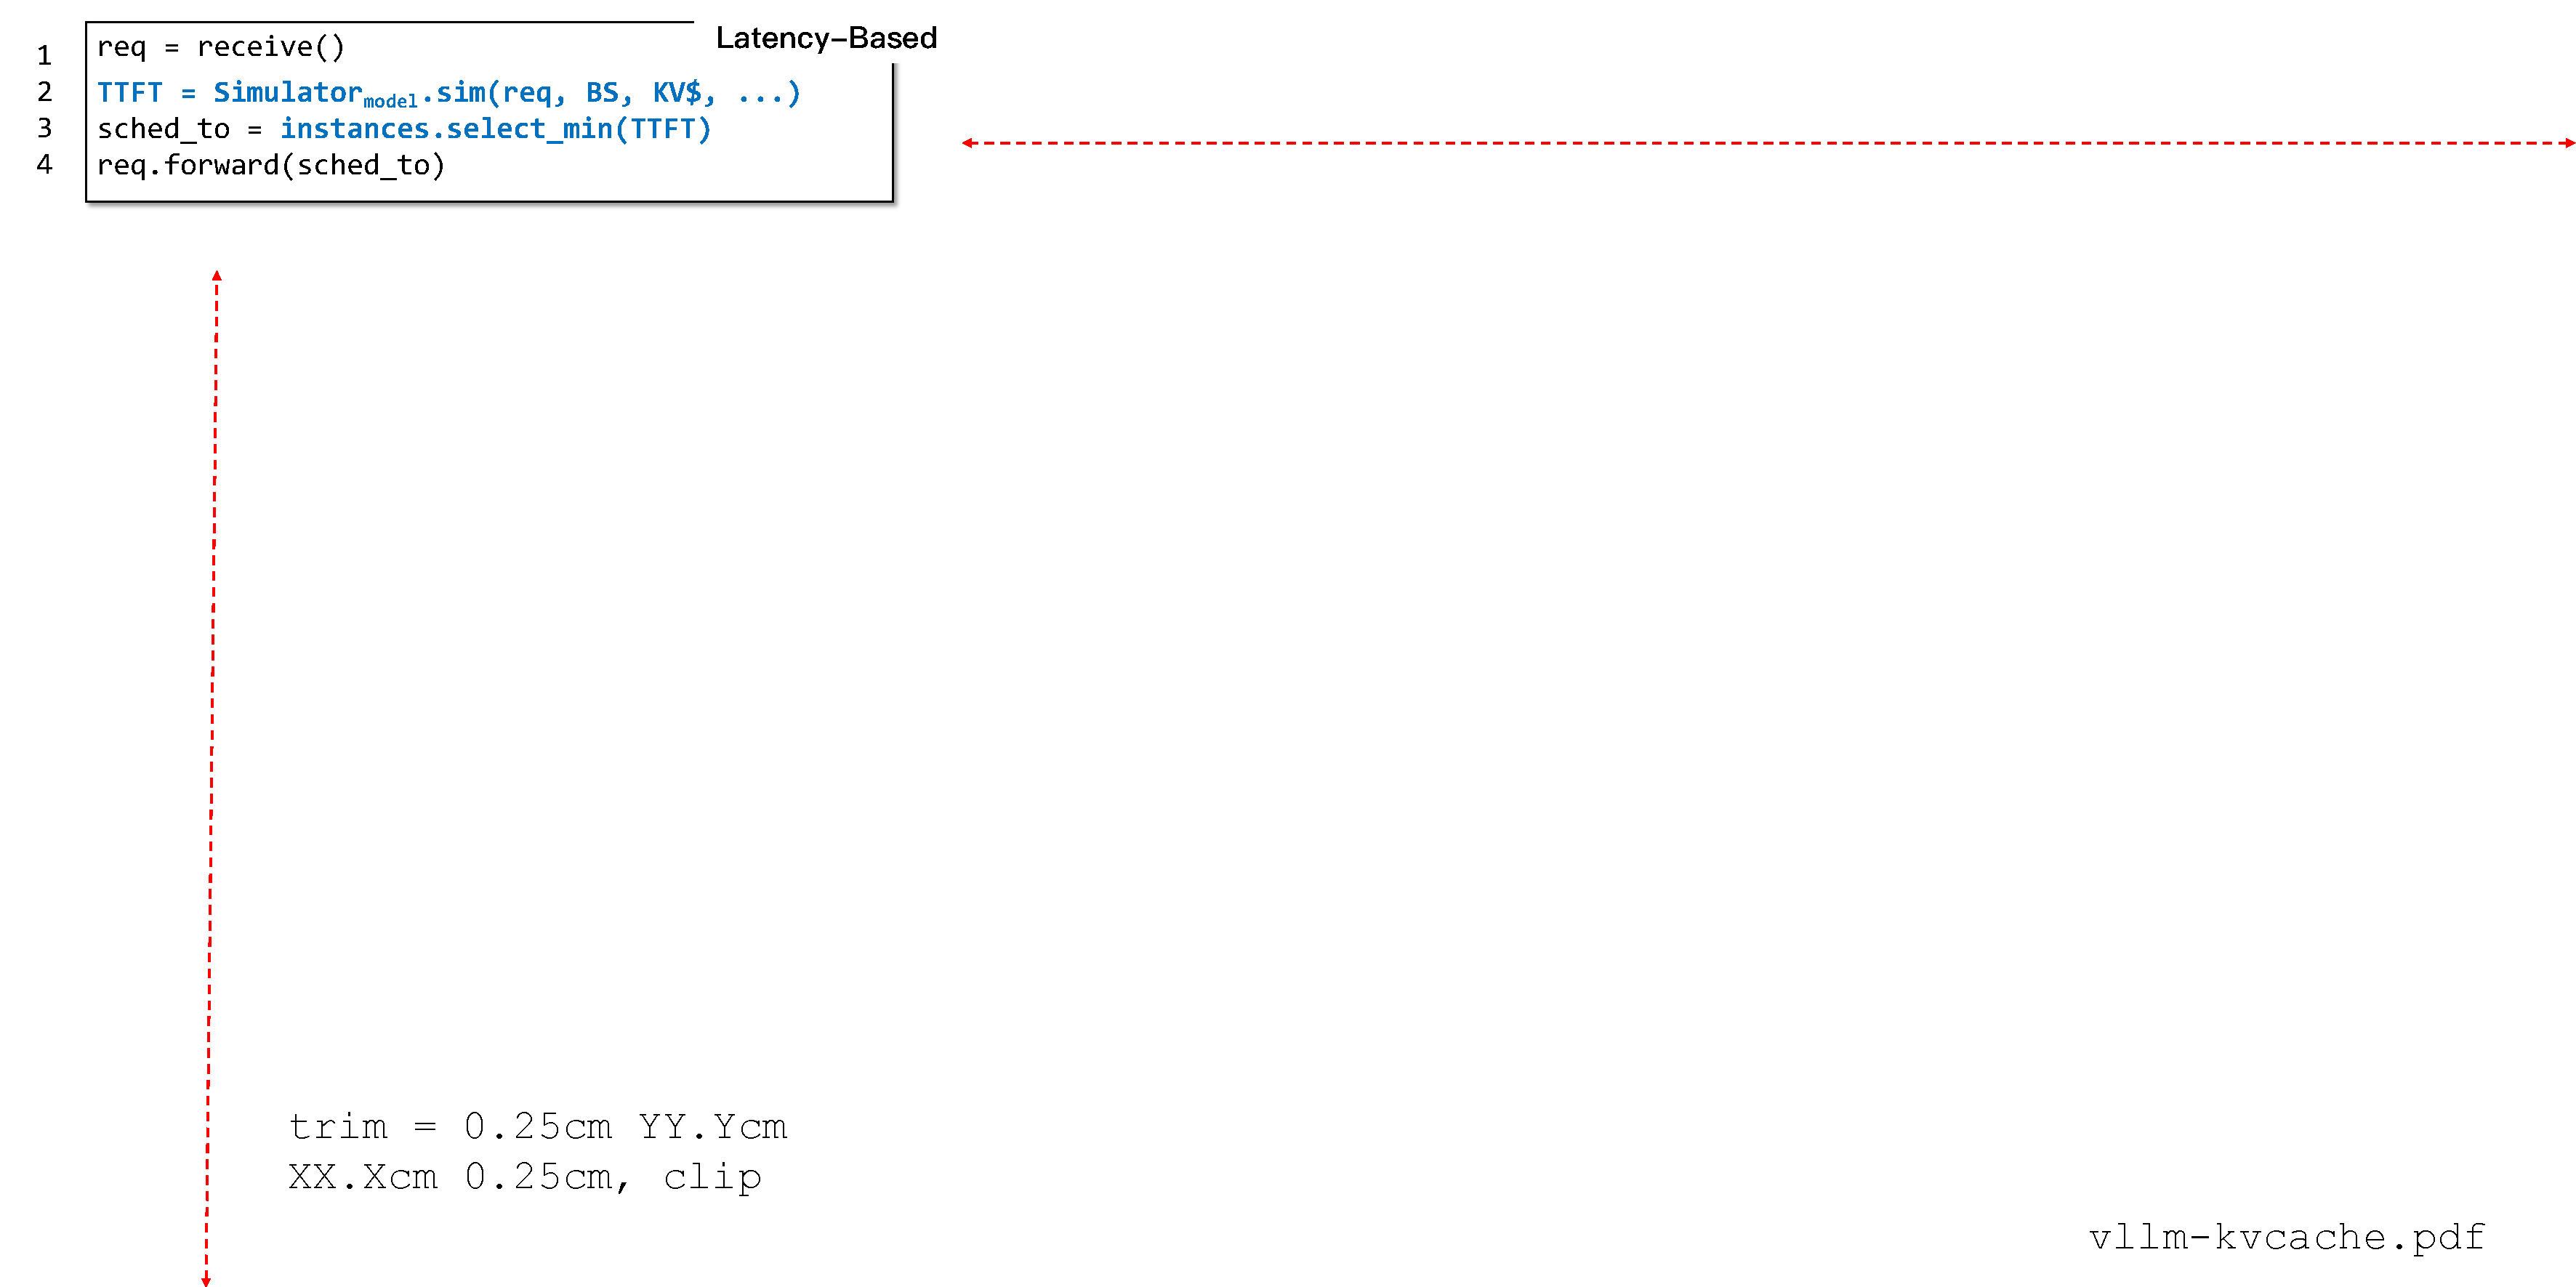
\includegraphics[width=0.96\linewidth, trim=0.25cm 25cm 38cm 0cm, clip]{figs/latency-based-v1.pdf} \\[6pt]
    \begin{minipage}{1\linewidth}
    \caption{\small{
        The pseudocode of simulation-based method for combining {\kvcache}-awareness and load balancing in LLM scheduling. 
        }}
    \label{fig:latency-based-scheduling}
    \end{minipage} \\[-10pt]
\end{figure}


\begin{figure*}[!t]
%    \hspace{1mm}
    \centering
%    \includegraphics[width=1\textwidth]{./figs/motiv/traces-v1.pdf}\\[-2pt]
    %  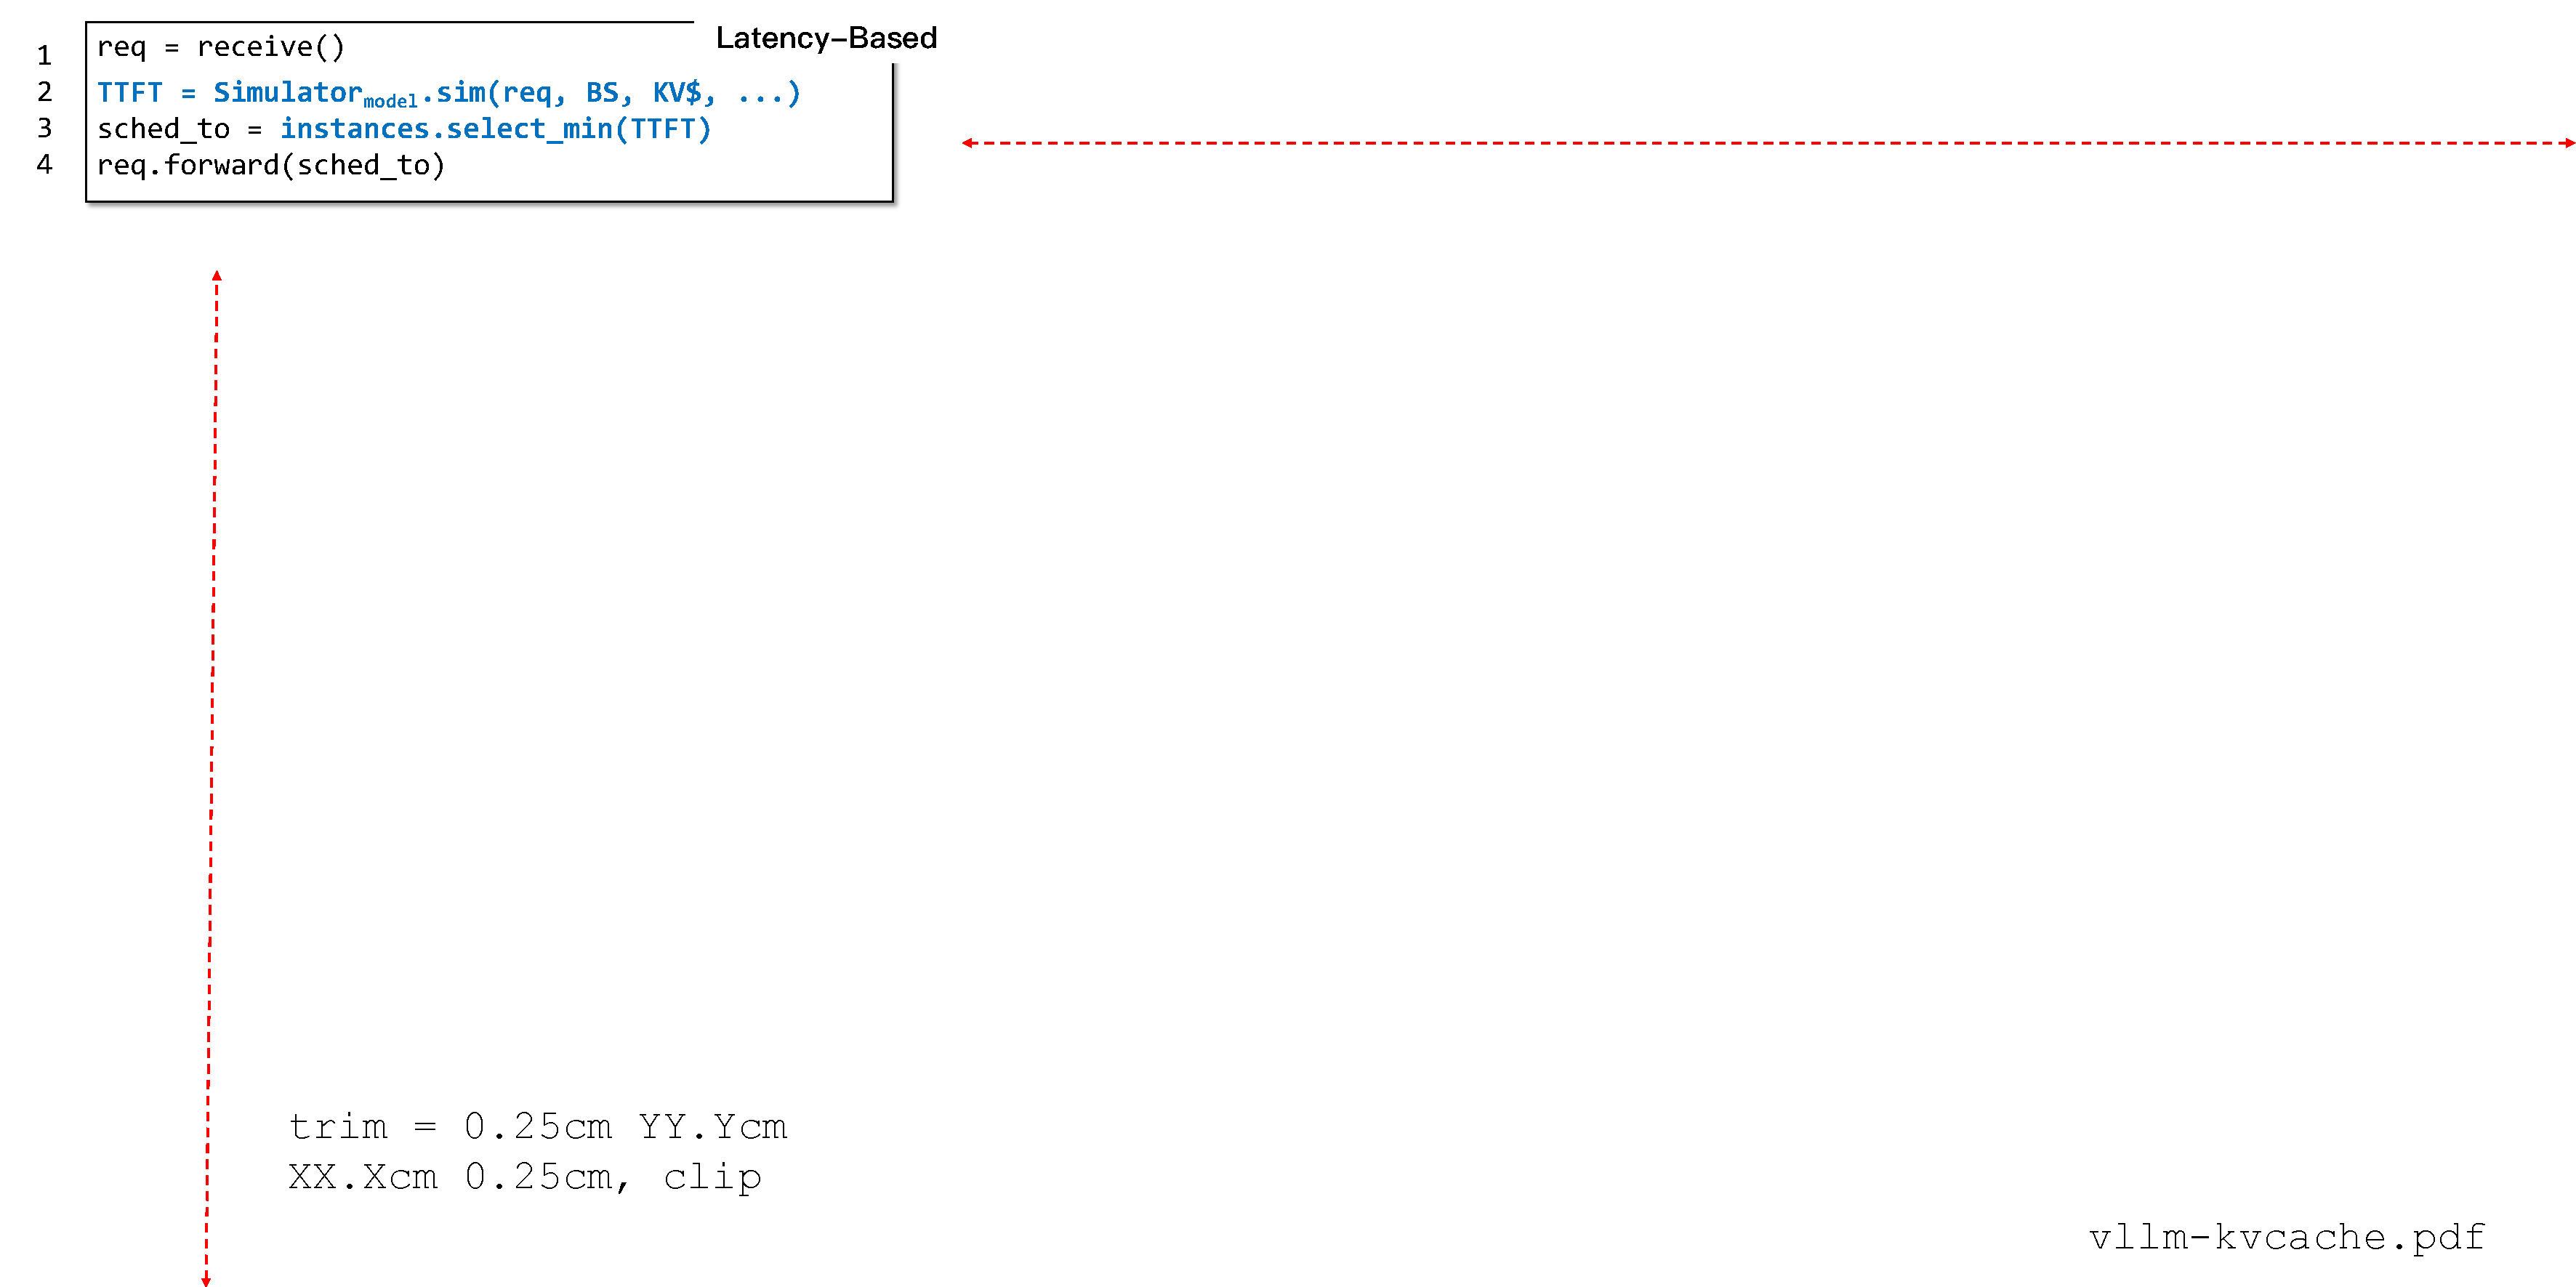
\includegraphics[width=0.96\linewidth, trim=0.25cm 14.5cm 41cm 0.25cm, clip]{figs/latency-based-v1.pdf} \\[-2pt]
    % \includegraphics[width=0.96\linewidth, trim=0.25cm -0.1cm 0cm 0.1cm]{figs/tuning/predictor-vs-wrong-predictor-e2e.pdf} \\[-2pt]
    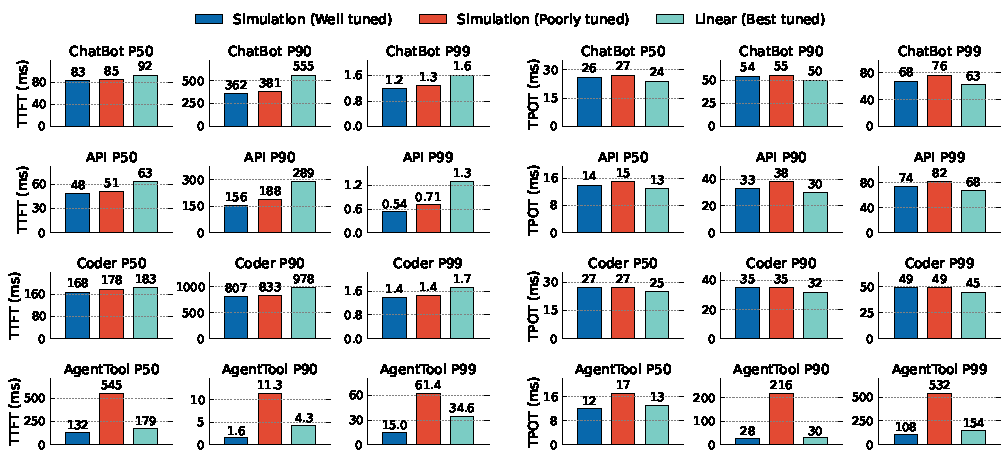
\includegraphics[width=0.85\linewidth]{figs/tuning/predictor-vs-wrong-predictor-v3.pdf} \\ 
    \begin{minipage}{1\linewidth}
    \caption{\small{
    An analysis of how performance varies with different simulator accuracy across
    four traces using a Qwen3-30B model.
        }}
    \label{fig:wrong-predictor-e2e}
    \end{minipage} \\[-10pt]
\end{figure*}

\begin{figure}[t]
    \centering
    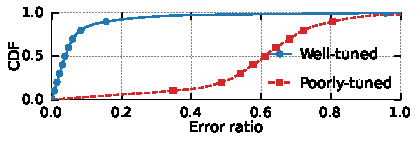
\includegraphics[width=0.85\linewidth]{figs/tuning/predictor-vs-wrong-predictor-accuracy.pdf} \\[-5pt]
    \caption{\small{   
    A comparison of a well-tuned simulator
    vs. a non-tuned one on ChatBot Trace with Qwen3-30B model. 
    }}
    \label{fig:predictor-accuracy-cdf}
\end{figure}

\nospacestitle{Methodology. \,}
Finally, simulation-based methods~\cite{305212, llm-d, DBLP:journals/corr/abs-2507-17769, DBLP:journals/corr/abs-2504-08784}
use the simulated serving time of a request when routing it to a specific instance as the routing score.
This is based on the observation that the execution of LLM requests is quite structured,
so it can be simulated accurately.
{\fig{fig:latency-based-scheduling}} shows the pseudocode of a typical simulation-based method~\cite{llm-d}:
after receiving a request,
the router first estimates the TTFT of routing the request to each instance via a simulator (e.g., VIDUR~\cite{DBLP:conf/mlsys/AgrawalKMPKGRT24}) (line 2),
and then routes the request to the instance with the lowest estimated TTFT (lines 3--4).
Note that simulation-based approaches typically estimate the TTFT instead of the end-to-end latency
because the end-to-end latency depends on the number of output tokens, which is unpredictable.


Simulation-based solutions can be viewed as a higher-order combination
of indicators that achieve {\kvcache}-awareness and load-balancing.
This is because the simulator must use the {\kvcache} state and batch size of each instance
as input features to accurately simulate the TTFT.
Here, we chose a simulation-based implementation 
similar to llm-d~\cite{llm-d}
 but with a retrofitted simulator from VIDUR~\cite{DBLP:conf/mlsys/AgrawalKMPKGRT24}---the 
state-of-the-art LLM instance simulator. 
Our retrofitting consists of two parts:
(1) we extend the simulator to consider {\kvcache}-aware execution by modeling the prefill phase with cache hits,
and (2) we re-implement it in Rust and enable parallel simulation to scale the online simulation to multiple instances. 
Without {\kvcache}-awareness, the simulation-based solution cannot outperform other counterparts,
similar to the observations we made in \textsection{\ref{sec:kvcache-aware}}.
Without Rust, the original Python-based implementation has considerable scheduling latency
and is not suitable for online scheduling.
We also have several optimizations to scale the simulator to hundreds of instances 
and we will leave the details to another paper as it is not the focus of this work. 
%Our implementation achieves similar or higher accuracy compared to the original one,
%thanks to the {\kvcache}-awareness.

We studied a state-of-the-art method and found that it
outperforms the linear-combination-based method in some traces,
as also shown in {\fig{fig:latency-based-scheduling}}.
Despite the improved performance, simulation-based methods still have two issues due to their complexity:

\stitle{Cons \#1. Development complexity due to per-model development and per-hardware tuning.  \,}
The performance of simulation-based methods is dependent on the accuracy of the simulator,
which is non-trivial to achieve in practice because
we need to consider both the model architecture and the hardware characteristics.
To quantify the impact of simulator accuracy on scheduling performance,
{\fig{fig:wrong-predictor-e2e}} presents the performance of
using well-tuned vs. non-tuned simulators on four traces when serving a Qwen3-30B model.
The poorly tuned simulator is one originally used for another model---Qwen2-7B,
while a well-tuned simulator is the one implemented specifically for Qwen3-30B.
{\fig{fig:predictor-accuracy-cdf}} measures the TTFT deviation when using
two simulators to serve a Qwen3-30B model compared with using vLLM.
We can see that a well-tuned simulator achieves much higher accuracy than an untuned one.
With a more accurate simulator, the TTFT and TPOT tail latency improve
by 75.6\% and 79.7\%, respectively.

While it is possible to develop simulators for each model for high scheduling performance, 
doing so incurs non-trivial development complexity
because the simulations 
highly depend on the model architecture---which is evolving rapidly
with new modules (e.g., linear attention~\cite{qwen3-next} and Engram~\cite{cheng2026conditionalmemoryscalablelookup}).
Meanwhile, for the same model, the hyperparameters of the simulator need to be tuned according to the hardware characteristics,
leading to further development efforts. 
%We can see that even with a well-tuned simulator, there are still about 10\% of requests with more than 20\% prediction error. 
%Such errors mainly come from 2 sources, request reordering at the vLLM API server, inaccuracies in the latency prediction. 

\stitle{Cons \#2. Still sub-optimal performance. \,}
Simulation-based methods still suffer from suboptimal performance,
especially for TPOT.
As shown in {\fig{fig:wrong-predictor-e2e}},
on the AgentTool trace, the TPOT tail latency is 71.1\% slower than that of the best linear-combination-based method.
We hypothesize that this is because some mispredictions of the simulator lead to load imbalance.
For example, in {\fig{fig:predictor-accuracy-cdf}}, we can see
that even with a well-tuned simulator, there are still about 10\% of requests with more than 20\% prediction error.
Such errors mainly come from two sources: request reordering at the vLLM API server,
and inaccuracies in latency prediction.
%and that is not recongnized by scheduler since the simulation-based methods are insensitive to changes in batch size.

\iffalse
\begin{figure}[!t]
    %\hspace{-3mm}
    \centering
    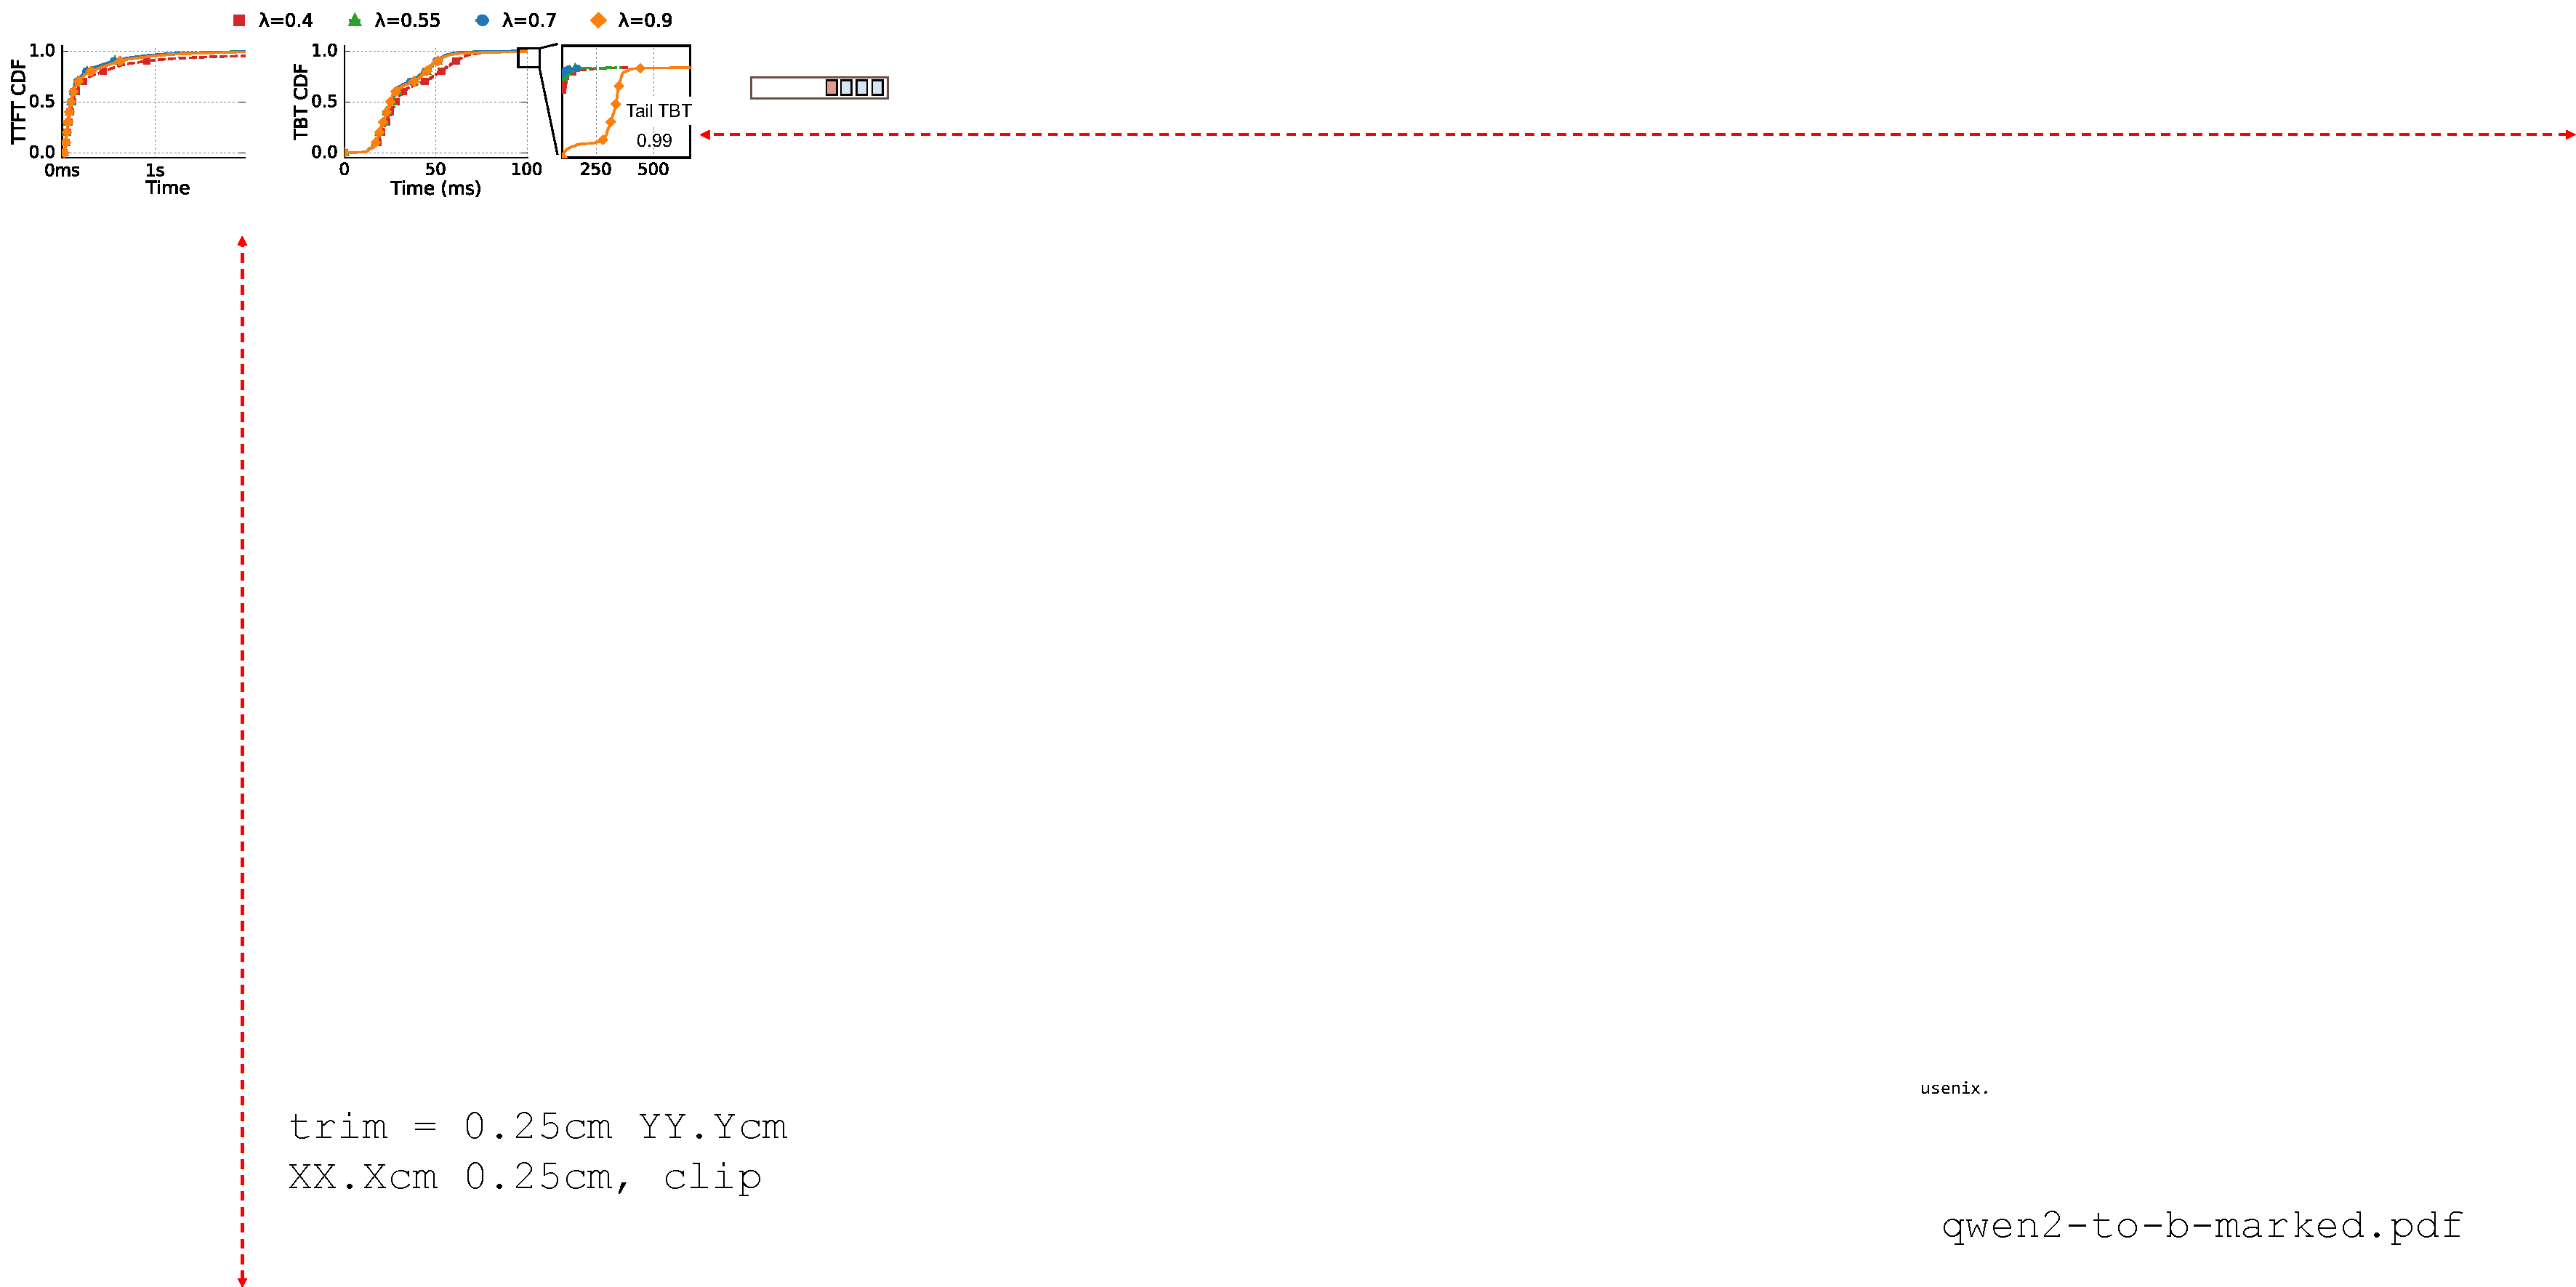
\includegraphics[width=1.02\linewidth, trim=0.25cm 24.55cm 43.75cm 0.25cm, clip]{figs/4-3-param-tuning/4-3-ptune-to-c-marked.pdf} \\[2pt]
    \begin{minipage}{1\linewidth}
    \caption{\small{Parameter tuning of KVCache hit ratio + batchsize policy on ChatBot(Qwen) trace}}
    \label{fig:lin-ptune-to-c}
    \end{minipage} \\[-10pt]
\end{figure} 

\begin{figure}[t]
    \centering
    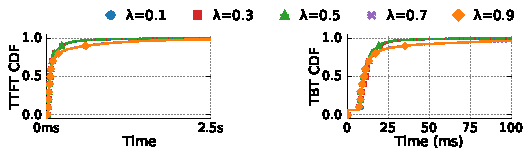
\includegraphics[width=0.8\linewidth]{figs/4-3-param-tuning/4-3-ptune-to-b-no-tail.pdf}
    \caption{\small{Parameter tuning of KVCache hit ratio + batchsize policy on Agent(Qwen) trace}}
    \label{fig:lin-ptune-to-b}
\end{figure}

\begin{figure}[t]
    \centering
    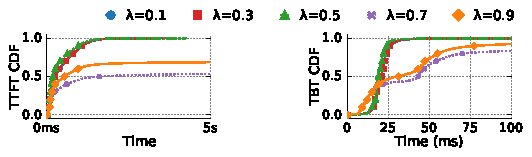
\includegraphics[width=0.8\linewidth]{figs/4-3-param-tuning/4-3-ptune-coder-no-tail.pdf}
    \caption{\small{Parameter tuning of KVCache hit ratio + batchsize policy on Coder trace}}
    \label{fig:lin-ptune-coder}
\end{figure}

\begin{figure}[t]
    \centering
    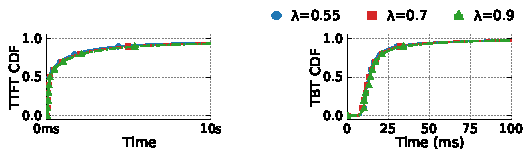
\includegraphics[width=0.8\linewidth]{figs/4-3-param-tuning/4-3-ptune-mooncake-tool-no-tail.pdf}
    \caption{\small{Parameter tuning of KVCache hit ratio + batchsize policy on ToolAgent(Kimi) trace}}
    \label{fig:lin-ptune-kimi-tool}
\end{figure}


% \begin{figure}[t]
%     \centering
%     \includegraphics[width=0.8\linewidth]{./figs/4-3-interference-aware/tpot_cdf_Least-Ptks_0_9_10_15_t0-1400.pdf}
%     \caption{\small{TPOT CDF in Least prefill tokens routing policy}}
%     \label{fig:tpot-least-ptkns}
% \end{figure}

% \begin{figure}[t]
%     \centering
%     \includegraphics[width=0.8\linewidth]{./figs/4-3-interference-aware/tpot_cdf_Mooncake_0_9_10_15_t0-1400.pdf}
%     \caption{\small{TPOT CDF in latency-prediction based routing policy}}
%     \label{fig:tpot-mooncake}
% \end{figure}

% \begin{figure}[t]
%     \centering
%     \includegraphics[width=0.8\linewidth]{./figs/4-3-interference-aware/batch_size_timeline_Least-Ptks_0_9_10_15.pdf}
%     \caption{\small{Batchsize timeline of the Least prefill tokens routing policy}}
%     \label{fig:bs-least-ptkns}
% \end{figure}


\begin{figure}[t]
    \centering
    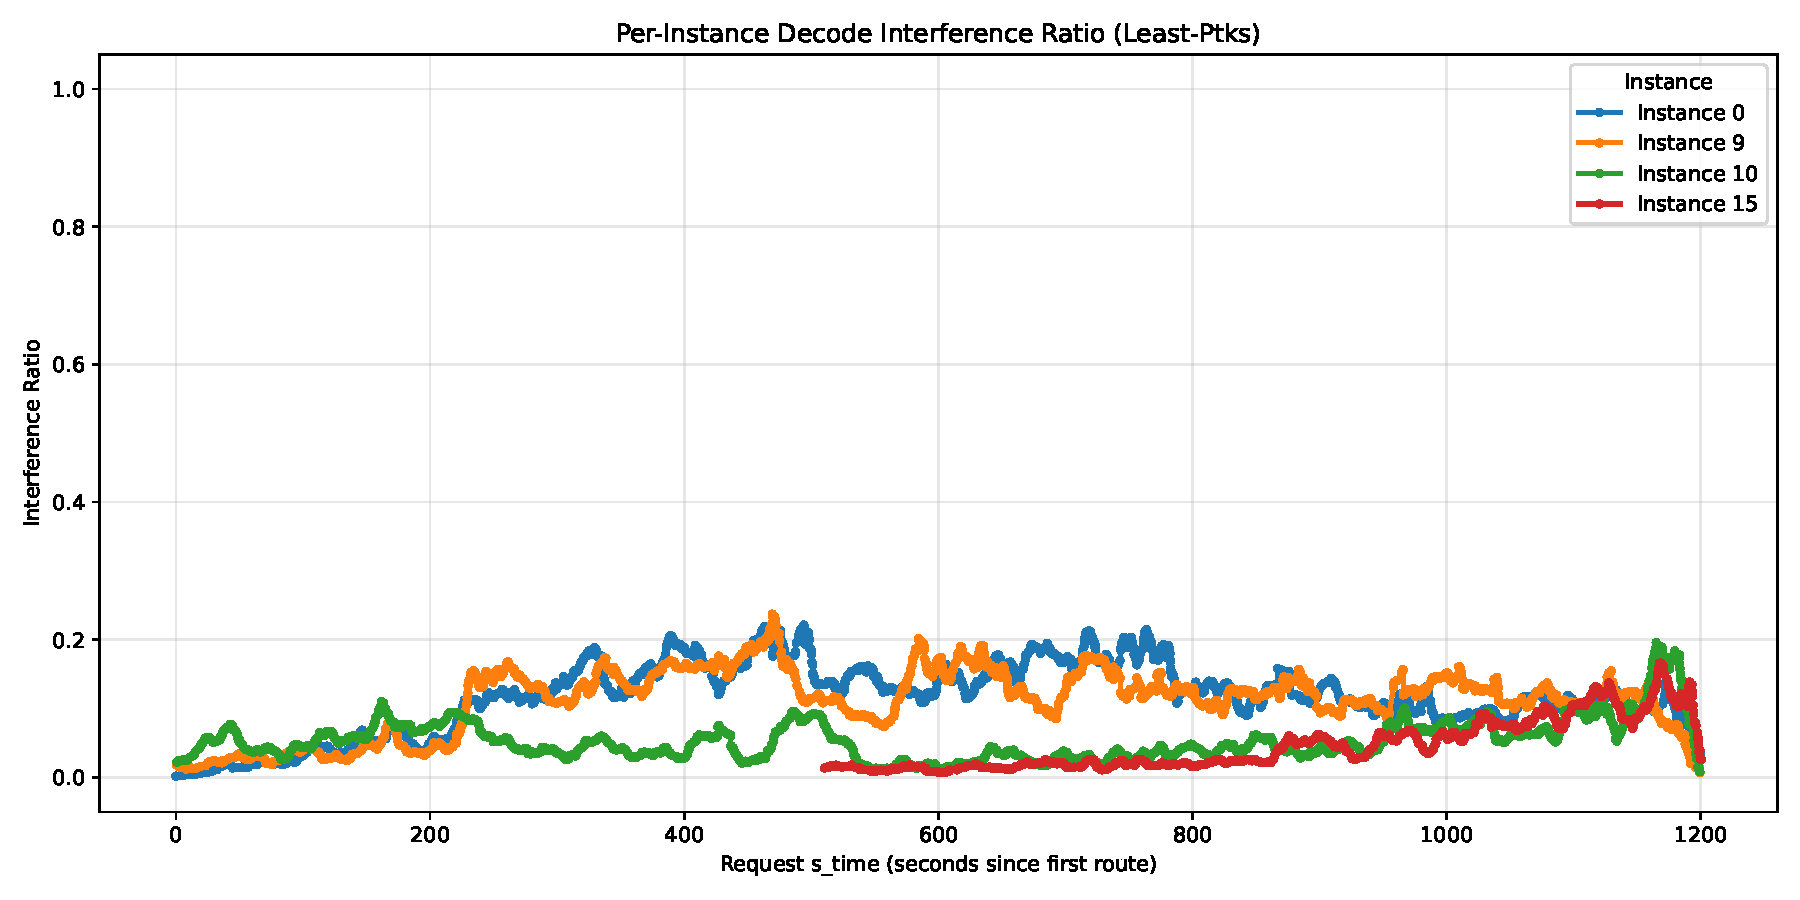
\includegraphics[width=0.8\linewidth]{./figs/4-3-interference-aware/interference_ratio_per_instance_Least-Ptks.pdf}
    \caption{\small{CP-Cycle of the Least prefill tokens routing policy}}
    \label{fig:bs-least-ptkns}
\end{figure}


\fi
